\documentclass[11pt]{article}
\usepackage{graphicx} % Required for inserting images
\usepackage{hyperref}
\usepackage{listings}
\usepackage{caption}
\usepackage{minted}
\usepackage{todonotes}
\usepackage[a4paper, total={6in, 8in},margin=1in,top=0.81in,bottom=1.25in]{geometry}
\usepackage{fancyhdr}
\usepackage{pdfpages}
\usepackage{sectsty}
\usepackage{fontspec}
\usepackage{multicol}
\usepackage{hyphenat}
\usepackage{polyglossia}

\newfontfamily{\cyrillicfont}{Liberation Serif}
\newfontfamily{\cyrillicfonttt}{Liberation Serif}
\setdefaultlanguage{serbian}
\sectionfont{\fontsize{24}{30}\selectfont}  % 24pt size, 30pt line spacing
\subsectionfont{\fontsize{18}{24}\selectfont}
\subsubsectionfont{\fontsize{14}{18}\selectfont}
\renewcommand{\listingscaption}{Изворни код}
\renewcommand{\listoflistingscaption}{Списак изворних кодова}
\pagestyle{fancy}
\fancyhf{}
\fancyfoot[L]{\fontsize{11}{13}\selectfont Алекса Бајат, Међурепрезентације изворног кода у фронтенду rustc компајлера}
\fancyfoot[R]{\newline\fontsize{11}{13}\selectfont \thepage}

\title{Међурепрезентације изворног кода у фронтенду rustc компајлера}
\author{Алекса Бајат}
\date{Мај 2025}

\begin{document}

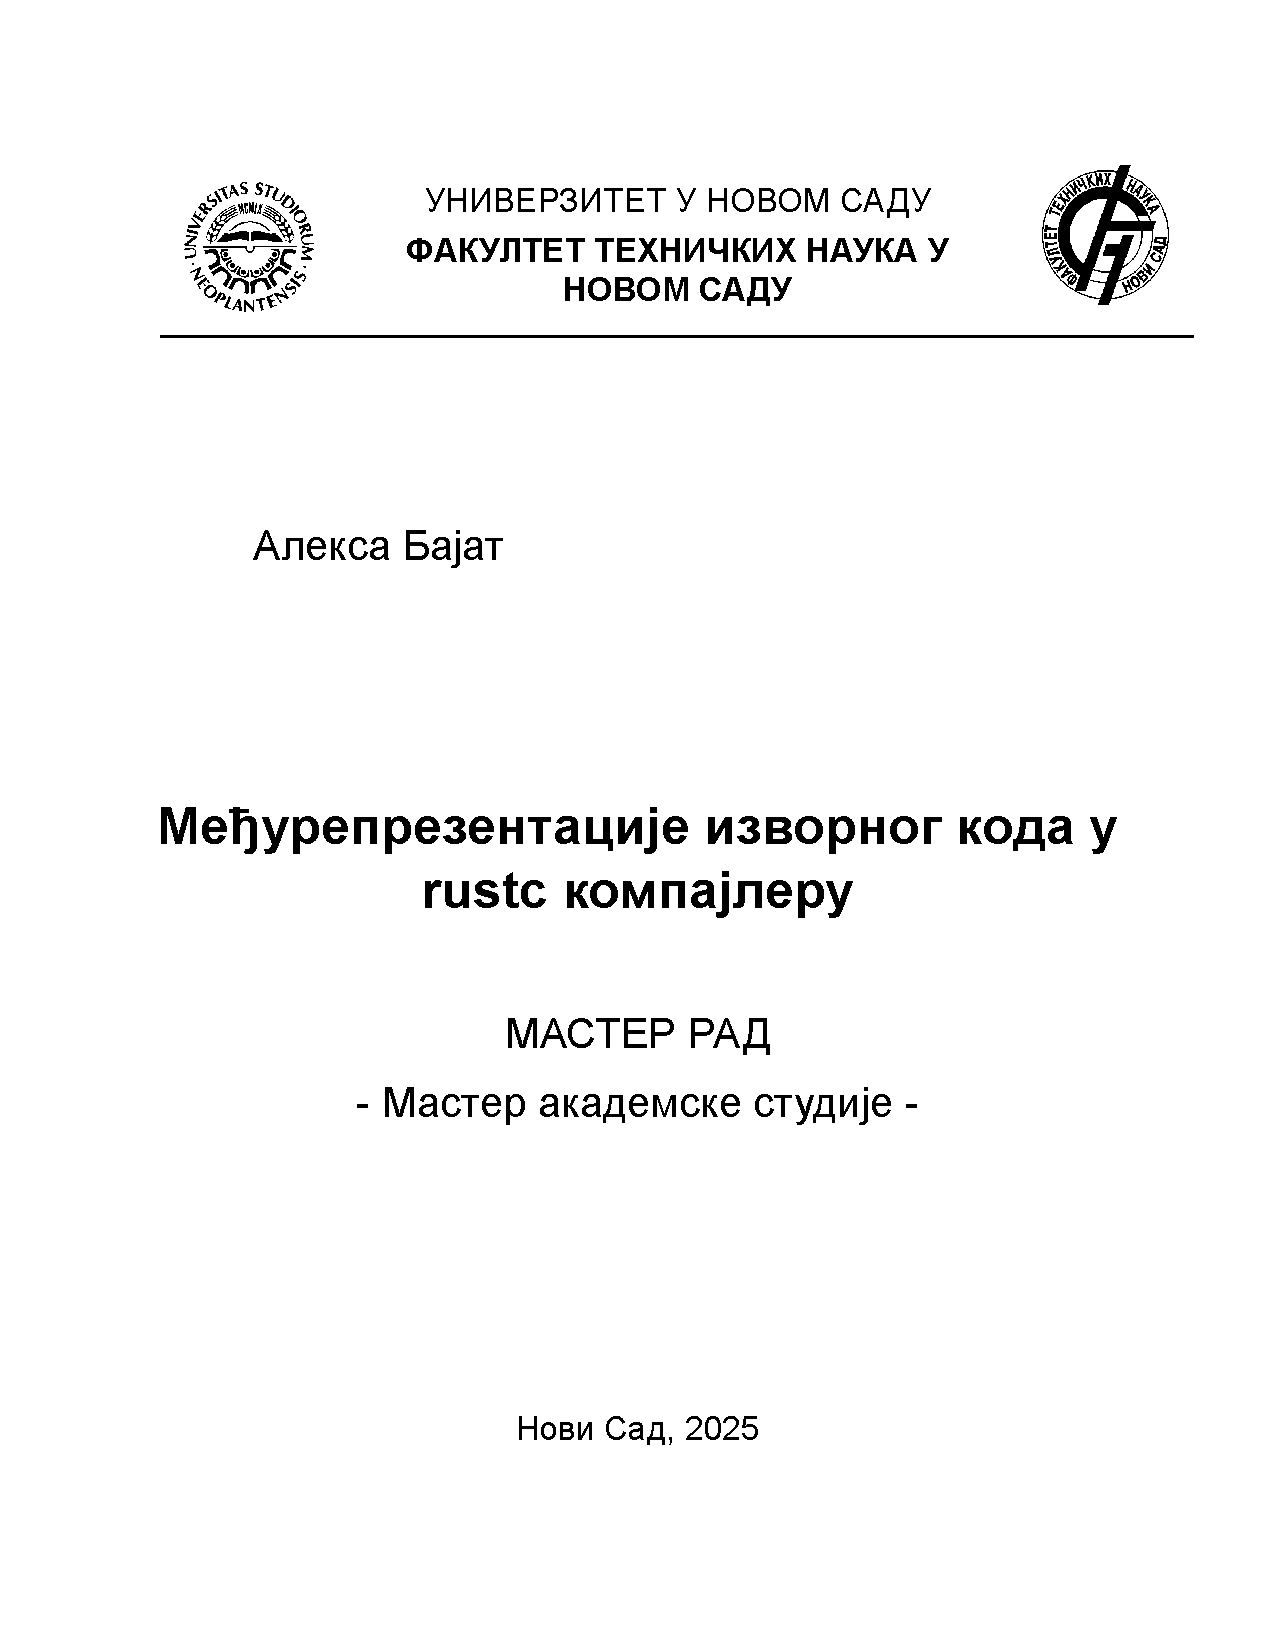
\includepdf[pages={1-4}]{MscTemplate.pdf}
\section{Spisak skraćenica}

\begin{enumerate}
    \item ASS - Apstraktno sintaksno stablo 
    \item MVN - Medjureprezentacija visokog nivoa
    \item TMVN - Tipizirana medjureprezentacija visokog nivoa
    \item MSN - Medjureprezentacija srednjeg nivoa
\end{enumerate}
\include{pages/toc.tex}
\section{Uvod}

Prilikom razvoja operativnih sistema, drajvera, bootloader-a i drugih kritičnih sistemskih softvera, koriste se jezici niskog nivoa kao što su C i C++.
Tokom godina Microsoft je uvideo da je preko 70\% bezbednosnih slabosti nastalo neadekvatnim rukovanjem memorijom [1]. Najčešći primeri su korišćenje memorije 
nakon oslobadjanja, višestruko oslobadjanje iste memorijske lokacije, nebezbedna aritemetika pokazivačima, curenje memorije i prepopunjavanje bafera.
Takođe sa stanovišta paralelnog programiranja, oba jezika zahtevaju pedantno rukovanje muteksima i semaforima jer u suprotnom nastaju novi problemi poput 
problema trke i problema medjusobnog čekanja. Problem trke nastaje kada dve ili više niti pokušavaju da izmene podatak istovremeno, pri čemu redosled izvršavanja 
utiče na ishod. Problem medjusobnog čekanja nastaje kada dve ili više niti čekaju jednu na drugu da oslobode resurse pri čemu se izvršavanje 
zaustavlja.

Programski jezik C nema ugrađene odbrambene mehanizme od prethodno navedenih problema. Pridržavanje C standardu otvara mogućnost za uporedo 
korišćenje GCC i Clang kompajlera čime se dobija uvid u relativno štura upozorenja od strane oba programska prevodioca.
Sa druge strane programski jezik C++ uprkos dodavanju primitiva kao što su \verb|unique_ptr|, \verb|shared_ptr| i \verb|weak_ptr|, i dalje zbog interoperabilnosti 
sa starijim standardima ili bibliotekama zahteva korišćenje sirovih pokazivača. Vremenom su se razvili softverski obrasci kao što je \verb|Scope-bound Resource Management|
koje nastoji da dobrim praksama umanji šansu da se problem prvobitno desi. Naime, korisnik jezika nije primoran da softverski obrazac upotrebi ili čak zna 
za njegovo postojanje.

Rust je programski jezik stvoren s jasnim ciljem: da reši probleme povezane sa memorijskom i paralelnom bezbednošću. 
Njegova podrazumevana upotreba garantuje bezbednost zahvaljujući robustom sistemu tipova, inovativnom načinu upravljanja memorijom i striktnog \verb|rustc| kompajlera.
Za razliku od C i C++ koji često daju nejasne poruke o greškama, Rust nudi izuzetno precizne dijagnostičke poruke koje tačno ukazuju na mesto 
greške i nude potencijalna rešenja.

Sa obzirom na značajne inovacije koje donosi Rust jezik, detaljno razumevanje njegovog internog funkcionisanja je od velikog značaja. Rust-ove garancije 
bezbednosti nisu magične, primarno proizilaze iz sistema pravila \verb|borrow-checker|-a, životnih vekova i osobina koje garantuju bezbednost nekog tipa 
u paralelnom okruženju. Rust nudi mnoge napredne funkcije kao što su makroi, unsafe kod, FFI (Foreign Function Interface) za interakciju sa C kodom. Detaljno razumevanje osnova jezika i njegovog internog funkcionisanja je preduslov za efikasno korišćenje ovih naprednih 
mogućnosti na siguran i efikasan način. Na primer, kada se koristi unsafe blok, programer preuzima odgovornost za bezbednost memorije, 
što zahteva duboko razumevanje načina na koji Rust obično to radi.

Zanimljivo je da je prva verzija Rust kompajlera bila napisana u O'Caml-u, ali su sve naredne verzije razvijene u samom Rust-u. 
Važno je napomenuti da je Rust zapravo samo frontend za LLVM. LLVM predstavlja skup modularnih i višekratno upotrebljivih tehnologija za izgradnju kompajlera. 
Rust se u potpunosti oslanja na LLVM za generisanje mašinskog koda, dok je kompletan frontend Rust-a napisan od nule.

Medjureprezentacije izvornog koda u Rust-u obuhvataju različite prikaze korisničkog koda koji omogu\hyp{}ćavaju ključne funkcionalnosti jezika, 
uključujući proveru tipova, dijagnostiku grešaka, automatsku dealo\hyp{}kaciju memorije i druge ergonomske i funkcionalne karakteristike.

\newpage

\section{Pozadina}

U ovoj sekciji obradjuje se pozadina iza \verb|Rust| jezika, zvaničnog menadžera paketa \verb|Cargo| i 
LLVM seta alata.

\subsection{Rust jezik}

\verb|Rust| je statički tipiziran jezik koji je nastao 2006. godine kao lični projekat \verb|Graydon| \verb|Hoare|-a, radnika kompanije 
Mozilla. Uvidevši potencijal jezika, Mozila je započela sponzorisanje projekta 2010. godine kada je jezik i javno 
predstavljen \cite{rust-language}. \verb|Rust| je jezik niskog nivoa koji se fokusira na memorijsku bezbednost
i bezbedan paralelizam bez oslanjanja na skupljač smeća (\verb|garbage| \verb|collector|). Skupljač smeća 
obično uvodi lakoću programiranja na uštrb nedeterminističkih performansi usled oslobadjanja memorije 
sa \verb|heap|-a, na memorijskim lokacijama gde je brojač referenci na nuli. U jezicima bez skupljača 
smeća obično postoji odredba koja se poziva da bi se dinamički alocirana memorija oslobodila. \verb|Rust|
jezik uvodi sasvim novi koncept u domen programskih jezika, pozajmljivač (\verb|borrow| \verb|checker|).
Pozajmljivač se zasniva na striktnoj primeni menadžmenta resursa u opsegu (\verb|scope-bound| \verb|resource| \verb|management|) 
od strane kompajlera. Ovo je softverski obrazac koji je preporučljivo koristiti u nebezbednim jezicima 
niskog nivoa. Naime u prirodi softverskog obrasca jeste da ga nije moguće primorati, osim ako nije direktno
integrisan u jezik kao što je slučaj sa jezikom \verb|Rust|. Ključan koncept koji se uvodi uz pozajmljivač 
jeste vlasništvo. Vlasništvo predstavlja dužnost da opseg koji direktno manipuliše memorijom (pristup memoriji nije 
pridobijen referencom) tu memoriju na kraju opsega oslobodi. 

U jeziku \verb|C| postoje dva načina deljenja 
memorije: preko vrednosti i preko reference (pokazivača). Deljenje preko vrednosti (kopija) je
podrazumevano. U \verb|Rust|-u deljenje preko vrednosti nije podrazu\hyp{}mevano ponašanje, već je osnovna akcija prenos vlasništva.
Deljenje preko vrednosti se može simulirati kloniranjem (funkcija \verb|clone|) koju prati prenos vlasništva.
Opseg u kome je memorija dodeljena varijabli validna 
se naziva životni vek. Vlasništvo onemogućuje brojne greške kao što su korišćenje nakon oslobadjanja i curenje 
memorije tj. aktivno vrši zabranu nedefinisanih stanja. Program se ne kompajlira uspešno ukoliko pravila 
vlasništva nisu zadovoljena. Izvorni kod \ref{lst:use_after_free_c} predstavlja C kod koji koristi memoriju 
nakon oslobadjanja. Uspešno se kompajlira ali prilikom izvršavanja vraća grešku. Sa druge strane u izvornom 
kodu \ref{lst:user_after_free_rust} predstavljen je isti koncept u \verb|Rust| jeziku. Funkcija 
\verb|drop| preuzmima vlasništvo nad memorijom 
i oslobadja je, simulirajući kraj opsega. Izvorni kod \ref{lst:user_after_free_rust} se neće 
uspešno kompajlirati jer se vrši pokušaj manipulacijom memorije nad varijablom kojoj je prošao životni vek.
Ujedno je demonstrirano da korisnik \verb|Rust| jezika ne mora da se stara o životnom veku varijable, isključujući
curenje memorije kao opcije.

\begin{multicols}{2}
    \begin{listing}[H]
    \begin{minted}{C}
int* pointer = malloc(sizeof(int));
*pointer = 5;
pointer = NULL;
free(pointer);
*pointer = 6; 
    \end{minted}
    \caption{Korišćenje nakon oslobadjanja - C}
    \label{lst:use_after_free_c}
    \end{listing}
    \columnbreak
    \begin{listing}[H]
    \begin{minted}{rust}
let mut a: Box<i32> = Box::new(5);
drop(a);
*a = 6;
    \end{minted}
    \caption{Korišćenje nakon oslobadjanja - Rust}
    \label{lst:user_after_free_rust}
    \end{listing}
\end{multicols}

U jeziku \verb|C++|, dobra praksa je pravilno označavati nepromenljivost reference ili vrednosti
unutar funkcija korišćenjem ključne reči \verb|const|, obaveštavajući budućeg korisnika funkcije 
o promenljivosti. U jeziku \verb|Rust|, promenljivost mora da se naznači eksplicitno upotrebom ključne 
reči \verb|mut|. Inverzija principa je omogućila daleko bolju čitljivost i razumevanje koda.

Bezbedni paralelizam je jedna od glavnih odlika \verb|Rust| jezika. Realizuje se pomoću osobina (\verb|trait|)
i vlasništva. Osobine su ugovor koji se postavlja nad strukturom i po funkcionalnosti liče na interfejse
u drugim jezicima. Glavna razlika je u fleksibilnosti. Osobine mogu da se implementiraju nad tipovima
koje nismo mi definisali, na primer iz drugih biblioteka. Razlog tome jeste baš u ključnoj reči ugovor.
Ako struktura zadovoljava ugovor koji osobina nalaže (obično ispunjenje drugih osobina ili
metoda) onda je osobina primenljiva nad strukturom. Ključne osobine koje realizuju bezbednost podataka
u paralelnom okruženju jesu \verb|Sync| i \verb|Send|. Tip je \verb|Send| ako je bezbedno poslati ga 
u drugu nit. Tip je \verb|Sync| ako ga je bezbedno deliti izmedju niti. Tipovi sačinjeni od drugih tipova koji
implementiraju \verb|Sync| i/ili \verb|Send| su automatski \verb|Sync| i/ili \verb|Send|. Skoro sve primitive
unutar \verb|Rust| jezika su \verb|Send| i \verb|Sync|. U bitnije izuzetke spadaju sirovi pokazivači jer nemaju
bezbednosne garancije, \verb|UnsafeCell| (samim time i \verb|Cell| i \verb|RefCell|) jer implementiraju
unutrašnju mutabilnost čime je tip rizik u vidu štetnog preplitanja, kao i \verb|Rc| (brojač referenci) 
jer je broj referenci deljen i nesinhronizovan. Uz \verb|std::marker|, \verb|Sync| i \verb|Send| su jedine osobine koje su 
deo samog kompajlera, a ne standardne biblioteke.

Atributi su zaglavlja koja pružaju dodatne informacije kompajleru. Atributi mogu biti spoljašnji ili 
unutrašnji \ref{lst:attributes}. Primenjuju se na brojne konstrukte unutar jezika kao što su eksterni blokovi,
funkcije, moduli i enumeracije. Atributi generišu kod, isključuju ili uključuju dijagnostiku, 
postavljaju limitacije i udeluju u testiranju. 

\begin{listing}[H]
\begin{minted}{rust}
// Spoljašnji atribut se primenjuje na tip koji sledi 
// nakon atributa koji pri tome nije atribut.
#[allow(dead_code)] 
fn main() {
    // Unutrašnji atribut.
    // Primenjuje se na vlasnika lokalnog opsega. 
    #![allow(unused_variables)]
    let x = 10;  
}
\end{minted}
\caption{Spoljašnji i unutrašnji atributi}
\label{lst:attributes}
\end{listing}

Makro sistem je jedan od najmoćnijih delova \verb|Rust| jezika. Makroi su kod koji generiše drugi kod i ovaj 
način programiranja se naziva metaprogramiranje. 
Korisni su da bi se smanjila količina koda koja mora da se održava, ali i da bi se izbeglo višestruko pisanje 
veoma sličnog koda (\verb|boilerplate|). Postoji četiri vrste makroa: deklarativni, funkcijski, proceduralni i atributski. 
Deklarativni i funkcijski su slični po prirodi, pozivaju se nalik običnim funkcijama ali u imenovanju imaju sufiks "!".
Deklarativni makroi moraju deterministički navesti broj parametara, dok funkcijski imaju proizvoljan broj parametara.
Jedan od najčešće korišćenih deklarativnih makroa jeste \verb|vec!| koji služi da smanji broj linija koda da bi se 
inicijalizovao vektor. Sa druge strane funkcijski makroi mogu da se koriste da bi se pisala sintaksa nekog drugog jezika, 
što je i česta pojava u \verb|Rust| bibliotekama koje pozivaju \verb|SQL| ili \verb|Python|.
Proceduralni makroi su makroi koji uvoze kroz predefinisani \verb|derive| atribut, dok atributski makroi generišu sasvim 
novi atribut. Glavna razlika izmedju njih jeste u fleksibilnosti. Proceduralni makroi rade na strukturama i enumeracijama,
dok atributski makroi mogu biti definisani da rade i nad drugim stavkama jezika poput funkcija.

\verb|Rust| jezik se odlikuje apstrakcijama bez cene. Osobina apstrakcija bez cene označava da koncepti 
višeg nivoa kao što su kolekcije i generički tipovi ne utiču na performanse programa prilikom njegovog izvršavanja.
\verb|Rust| omogućava ovu karakteristiku putem monomorfizacije. Monomorfizacija je proces putem kojeg se kreira 
kopija generičkog koda za svaki konkretan tip koji koristi generički kod tj. generički kod se pretvara u 
negenerički kod. Naime ovaj proces povećava veličinu krajnjeg izvršnog fajla i produžava vreme kompajliranja.
Generičke strukture mogu da imaju najveći uticaj na veličinu izvršnog fajla. Problem se amortizuje 
tako što se ne generišu metode za konkretan tip ako ih isti ne koristi u izvornom kodu.


\newpage
\subsection{Cargo}

U Rustu, \verb|Crate| je najmanja jedinica organizacije koda. Postoje dva osnovna tipa, izvršni programi i biblioteke.
Izvršni programi sadrže \verb|main| funkciju i mogu da se izvršavaju. Biblioteke se ne izvršavaju i nemaju potrebu za \verb|main|
funkcijom već pružaju funkcionalnosti koje se mogu koristiti u drugim \verb|Crate|-ovima. 

Skoro svaki modreni jezik dolazi sa jednim ili više menadžera paketa (biblioteka). Zvanični menadžer paketa u \verb|Rust|
ekosistemu se naziva \verb|Cargo|. Glavni zadatak mu je da beleži zavisnosti programa tako da je moguće rekreirati 
program na deterministički način. Uvode se \verb|Cargo.lock| i \verb|Cargo.toml|
fajlovi. \verb|Cargo.toml| je manifest fajl koji održava korisnik. Sastoji se meta podataka poput naziva i verzija kao i spiska paketa sa korisnički definisanim 
verzijama (ili opsegom verzija) koji se trenutno koriste u programu. Pored verzije, paketi mogu da imaju funkcionalnosti koje korisnik mora eksplicitno da navede ukoliko su potrebni.
\verb|Cargo.lock| se generiše nakon koraka kompajliranja ali ga je moguće izgenerisati kroz \verb|cargo| \verb|generate-lock| komandu.
\verb|Cargo.lock| omogućava da se pri kompajliranju programa na potenicjalno različitim mašinama koriste identični paketi praćenjem tačne verzije svakog pojedinačnog paketa.

\verb|Cargo| dobavlja zavisnosti iz registra. Registar sadrži indeks u kome se nalazi lista dostupnih \verb|Crate|-ova. Podrazumevani javni registar je \verb|crates.io|, ali je moguće 
konfigurisati sopstveni registar koji je proizvoljne vidljivosti. Jedan \verb|Crate| može koristiti zavisnosti iz različitih registara. Ukoliko se \verb|Crate| nalazi u registru koji nije 
podrazumevani u \verb|Cargo.toml| fajlu se za tu zavisnost definiše \verb|registry| atribut.

\verb|Cargo| je otporniji od menadžera paketa iz drugih ekosistema jer nije moguće brisati verzije jednom kada je paket objavljen na javnom registru. 
Ovaj pristup sprečava napade lanca snabdevanja kao što se desilo u \verb|JavaScript| menadžeru paketa \verb|NPM|. Paket \verb|left-pad| 
je sačinjen od 11 linija koda koji dodaje specificiranu količinu razmaka sa leve strane niza karaktera. Iako je paket trivijalan, mnoge biblioteke koje 
su masivno korišćene su direktno ili indirektno zavisile od njega. Problem je nastao kada je kreator \verb|left-pad| paketa obrisao 
paket sa repozitorijuma poremetivši ogroman deo ekosistema. U softveru otvorenog koda napadi lanca snabdevanja postaju sve češći (preko 700\% povišena učestalost
iz godine u godinu) i zbog toga regulatorne uprave rade na standardizaciji menadžera paketa ne bi li se ovakvi napadi sprečili \cite{supply-chain}.

Nekada je \verb|Crate|-u neophodno da kompajlira ili \verb|link|-uje neki kod koji nije napisan u Rust-u, na primer C kod. Koristeći poseban fajl \verb|build.rs| u korenskom direktorijumu 
projekta moguće je definisati skriptu koju će \verb|rustc| da kompajlira i izvrši pre kompajliranja ciljanog \verb|Crate|-a. Podrazumevano je da se skripta izvršava pred svaku kompilaciju,
ali je moguće definisati putanju ili promenljivu okruženja prilikom čije promene će se skripta ponovo (sledeći put kada se kompajlira \verb|Crate|) izvršavati.

\verb|Cargo| pored distribuiranja paketa pruža razne olakšice i automatizacije u odnosu na sirovo korišćenje \verb|Rust| kompajlera. 
Komanda \verb|cargo init| se koristi da bi se jednostavno inicijalizovao novi \verb|Crate| zajedno sa \verb|Cargo.toml| fajlom. 
Komande \verb|cargo| \verb|add| i \verb|cargo| \verb|remove| dodaju i brišu paket iz \verb|Cargo.toml| fajla.
Komanda \verb|cargo| \verb|check| kompajlira trenutni \verb|Crate| bez generacije koda (bez upotrebe LLVM-a) što je značajno brže 
od pokretanja \verb|cargo| \verb|build| koji i generiše kod. Ovo je korisno jer je većinski deo dijagnostike zasnovan 
na koracima pre generisanja koda. Komanda \verb|cargo| \verb|run| konstriše paket i izvršava ga. Ovo je značajno jer u većini slučajeva korisnik želi da pokrene program nakon što je 
napisao izmenu i izbegava \verb|CLI| gimnastiku dolaska do \verb|/target| foldera i pokretanja izvršnog fajla. 
Komanda \verb|cargo| \verb|test| pokreće sve \verb|unit| testove koji se definišu upotrebom atributa \verb|test| nad funkcijama.
Budući da je \verb|Cargo| delom apstrakcija nad \verb|rustc| kompajlerom i da je \verb|rustc| izuzetno konfigurabilan, koristi se komanda \verb|cargo| \verb|rustc|
koja prima dodatne kompajlerske opcije.

\newpage

\subsection{LLVM projekat}

Generisanje koda je jedan od najtežih zadataka prilikom kreiranja novog kompajlera. Izvorni kod koji 
korisnici pišu se prevodi u mašinski kod i pre svega mora biti tačan. Pored tačnosti cilj prilikom 
dizajniranja generatora koda jeste laka implementacija, testiranje i održavanje.
Prilikom prevodjenja obično postoji 
više medju reprezentacija izvornog koda sa ciljem da validira i optimizuje izvorni kod. Medju reprezentacije 
se svrstavaju u \verb|frontend| ili u \verb|backend|. \verb|Frontend| ima za zadatak da skenira, parsira 
i prevede izvorni kod u relativno nisku medju reprezentaciju. \verb|Backend| stoga može da pretpostavi 
da su sve statičke sintaktičke i semantičke greške detektovane i da su tipovi i njihove konverzije
obradjene na osnovu čega optimizuje i generiše kod za ciljanu arhitekturu.

LLVM projekat je skup modularnih i ponovo iskoristivih kompajlerskih tehnologija \cite{llvm}. Pod okriljem \verb|LLVM|-a
se nalaze brojni projekti. Glavni projekat je \verb|LLVM| \verb|Core| unutar koga je specificirana \verb|LLVM|
medju reprezentacija (\verb|LLVM| \verb|IR|) na kojoj se zasniva modularnost. Nad \verb|LLVM| medju reprezentacijom
je implementiran optmizator čiji kod se prosledjuje generatoru (\verb|backend|-u) koda cljane arhitekture. Samim time 
bilo koji \verb|frontend| koji se napiše tako da je krajnji izlaz \verb|LLVM| \verb|IR| može da iskoristi 
ostale delove kompajlera bez ikakvih dodatnih izmena \ref{lst:llvm_modular}.

\begin{listing}[H]
\begin{center}
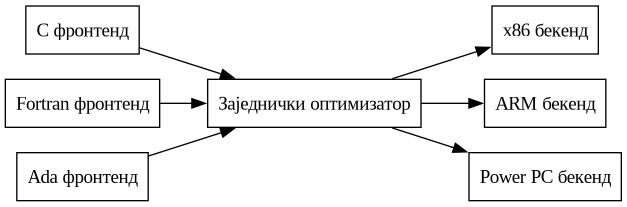
\includegraphics[width=5in, height=1.6in]{assets/images/modern_compiler_design.png}
\end{center}
\caption{Modularnost LLVM-a}
\label{lst:llvm_modular}
\end{listing}

Postoje brojne vrste optimizacije koje se mogu izvršiti nad izvornim kodom. Optimizacije se obično svode 
na tri osnovna koraka, pronalazak šablona koji se treba transformisati, validirati da li je bezbedno primeniti 
transformaciju i izvršavanje transformacije \cite{oss-architecture}. Optimizacije u \verb|LLVM| optmizatoru su modularne i izvršavaju 
se nad \verb|LLVM| medju reprezentacijom. Svaka \verb|LLVM| optmizacija je napisana kao \verb|C++| klasa koja 
nasledjuje \verb|Pass| (prolazak) klasu. Većina prolazaka je napisana u jedanom \verb|.cpp| fajlu.
Stoga otvara se mogućnost da se dodaju optimizacije specifične za jezik. Svaki prolazak se kompajlira u jedan 
ili više relokatabilnih objekata, (\verb|.o|) fajlova koji se potom grupišu u arhivne (\verb|.a|) fajlove. Objektni fajlovi 
su mašinski kod pre procesa linkovanja. Linkovanje je proces skupljanja i kombinovanja relokatabilnih objektnih fajlova
u jedan izvršni objektni fajl. Prilikom linkovanja nekog \verb|.o| fajla sa \verb|.a| fajlom linker će 
za svaki do tada nespojen simbol probati da nadje vezu u svim \verb|.o| fajlovima arhive.

\verb|LLVM| generator koda je odgovaran za prevodjenje \verb|LLVM| medju reprezentacije u mašinski kod ciljane 
arhitekture. Idealno za svaku arhitekturu postojao bi specifičan kod za prevodjenje, ali u isto vreme 
svi generatori rade vrlo sličan posao. Slično kao i kod optimizacije proces generisanja koda se deli u prolaske,
izbor seta instrukcija, način alokacije registara, planiranje (\verb|scheduling|), optimizacija rasporeda 
koda i generisanje asemblerskog koda. Pri kreiranju generatora za novu ciljnu arhitekturu svaki od ovih prolazaka
može ponovo da se iskoristi, modifikuje ili potpuno zameni.

\verb|LLVM| medju reprezentacija se veoma efikasno serijalizuje u i deserializuje iz \verb|LLVM| bitkoda. 
Ova efikasnost otvara mogućnost za optimizaciju u vreme linkovanja \ref{lst:link_time_opt}. To je još jedan set optimizacionih prolazaka 
koji dodatno poboljšava kranji mašinski kod. Linker prepoznaje da se u \verb|.o| fajlovima nalazi 
\verb|LLVM| bitkod umesto mašinskog koda, učitava ih u memoriju, linkuje ih, a potom izvršava \verb|LLVM|
optimizator nad mnogo većom celinom koda, omogućavajući daleko agresivnije optimizacije. 
Ova opcija se uključuje dodavanjem \verb|-O4| opcije komandne linije. 

\begin{listing}[H]
\begin{center}
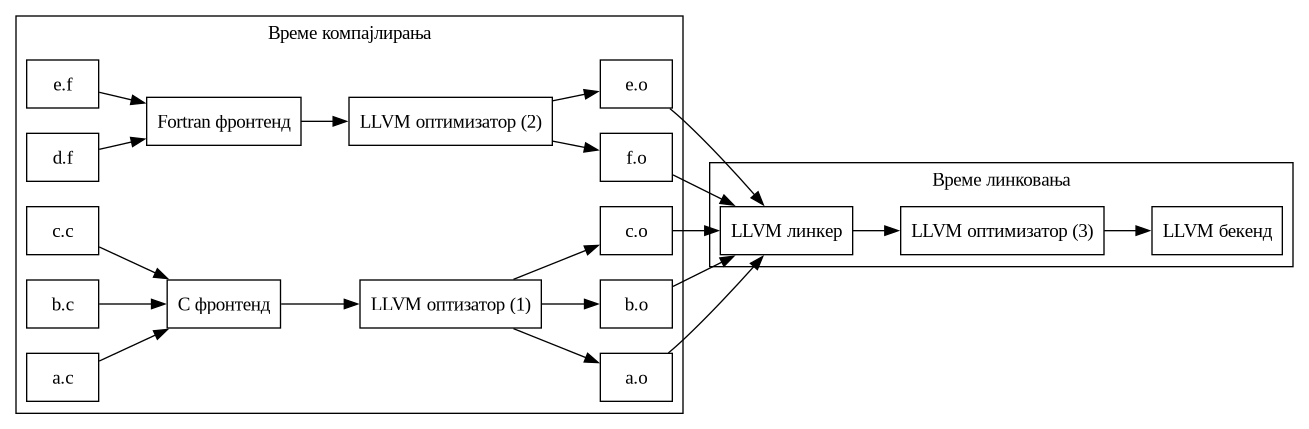
\includegraphics[width=6in, height=2.2in]{assets/images/link_time_optimization.png}
\end{center}
\caption{Optimizacija u vreme linkovanja}
\label{lst:link_time_opt}
\end{listing}

\verb|LLVM| medju reprezentacija podesća na asemblerski jezik. Strogo je tipiziran i poseduje jednostavne 
tipove poput celih brojeva, brojeva sa pokretnim zarezom, pokazivača i struktura. Jedna od glavnih razlika 
u odnosu na asembler jeste to što ne koristi ograničeni broj imenovanih registara već koristi beskonačan 
skup promenljivih koje se definišu sa \verb|%| prefiksom. Neki detalji mašine su apstrahovani od korisnika 
poput poziva funkcija (\verb|call|) i vraćanja vrednosti (\verb|ret|) \ref{lst:llvm_ir}.

\begin{listing}[H]
\begin{minted}{llvm}
define i32 @add2(i32 %a, i32 %b) {
entry:
  %tmp1 = icmp eq i32 %a, 0
  br i1 %tmp1, label %done, label %recurse

recurse:
  %tmp2 = sub i32 %a, 1
  %tmp3 = add i32 %b, 1
  %tmp4 = call i32 @add2(i32 %tmp2, i32 %tmp3)
  ret i32 %tmp4

done:
  ret i32 %b
}
\end{minted}
\caption{LLVM medju reprezentacija}
\label{lst:llvm_ir}
\end{listing}

\verb|Rust| jezik je \verb|frontend| nad \verb|LLVM|-om. Postoji puno olakšica u ovom pristupu.
\verb|Rust| tim ima cilj da izgeneriše pravilnu \verb|LLVM| medju reprezentaciju, na osnovu koje 
\verb|LLVM| izvršava optimizacione prolaske i generiše kod. Greške prilikom generisanja koda ne mora da 
održava \verb|Rust| tim, što značajno smanjuje količinu ljudi koja aktivno mora da bude uključena u razvoj. 
Svaka ciljna distribucija (arhitektura) koju \verb|LLVM| podržava automatski podržava i \verb|Rust|. Optimizacije se ne moraju 
posebno pisati i održavati jer \verb|LLVM| već poseduje značajan broj čestih optimizacija. \verb|Rust| 
omogućava kompajliranje na osnovu više \verb|LLVM| verzija, poslednja glavna verzija je uvek podržana,
i obično su podržane jedna ili dve ispod nje.

\section{Rust kompajler}

Rust kompajler u svakom trenutku poseduje tri glavne verzije skupa alata (\verb|toolchain|): stabilna, beta i noćna (\verb|nightly|) verzija.
Stabilna verzija kompajlera je bezbedna i preporučena za produkcionu upotrebu. Beta verzija sadrži funkcionalnosti
koje se usvajaju u narednoj stabilnoj verziji. Noćna verzija je verzija kompajlera koja se 
proizvodi svaku noć, sa svim najnovijim netestiranim promenama. Kapija funkcionalnosti je mehanizam bezbednosti
koji onemogućava da eksperimentalne (nestabilne) funkcionalnosti slučajno završe u produkciji. 
Kapija je definisana na osnovu stanja kapije, naziva funkcionalnosti, verzije, broja zahteva za povlačenjem
(\verb|pull| \verb|request|) i opcionog komentara.
Stanje kapije funkcionalnosti može biti nestabilno, obrisano ili prihvaćeno i nekompletirano. Nekompletirano 
stanje unutar kapije daje do znanja korisniku noćne verzije ili drugim saradnicima da je nestabilna funkcionalnost 
u razvoju.  Nestabilne kapije onemogućavaju da stabilna i beta verzija kompajlera kompajliraju 
dati segment koda (ignoriše se).  Samim time razvoj je direktno 
usmeren ka noćnoj verziji koja je pod nadzorom celokupnog Rust tima. Obrisane kapije se ne brišu fizički iz koda,
već se status kapije promeni u obrisan uz komentar sa razlogom. Na ovaj način se čuva istorija pokušanih 
funkcionalnosti sa razlozima koji su uzrokovali brisanje. U slučaju da se sličan zahtev ponovo javi, retrospektiva
služi kao moćan alat koji će idealno upozoriti saradnike i preusmeravati ih na bolji pravac.

\begin{listing}[H]
\begin{minted}{rust}
    (incomplete, pub_restricted, "CURRENT_RUSTC_VERSION", Some(32409)),
    (unstable, pub_restricted, "CURRENT_RUSTC_VERSION", Some(32409))
    (accepted, pub_restricted, "CURRENT_RUSTC_VERSION", Some(32409)),
    (removed, pub_restricted, "CURRENT_RUSTC_VERSION", 
    Some(32409), Some("Removed because.."))
\end{minted}
\caption{Kapija funkcionalnosti}
\label{lst:rustup_set}
\end{listing}

Svaka funkcionalnost prolazi kroz dugačak proces provera pre nego 
što se usvoji. Ukoliko funkcionalnost zahteva promene koje nisu reorganizacija, refaktorisanje, dokumentovanje
i slično, kreira se zahtev za komentare (\verb|RFC|) koji detaljno objašnjava važnost funkcionalnosti i 
pregled implementacionih detalja sa visine. U suprotnom ovaj segment se preskače. Stejkholderi kao što je Rust kompajler tim, ali i sama Rust zajednica 
ima pravo da vaga o potencijalnim implikacijama koje funkcionalnost donosi. Odobravanje zahteva znači početak 
razvoja ali ne garantuje usvajanje. Ukoliko je funkcionalnost razvijena, pokrivena testovima, 
bez značajnih primedbi, bilo koji saradnik može pokrenuti zahtev za stabilizaciju. Zahtev je konstituiran iz 
četiri dela: dokumentacionog \verb|pull| \verb|request|-a, stabilizacionog izveštaja, 
perioda finalnog komentara i stabilizacionog \verb|pull| \verb|request|-a.

Dokumentacija funkcionalnosti koja se stabilizuje se briše iz nestabilne knjige \cite{unstable} i ažurira se 
dokumentacija namenjena korisnicima jezika. Korisnici povlače informacije iz različitih delova dokumentacije,
naime najbitnije je detljno ažurirati knjigu referenci \cite{rust-reference} koja opisuje svaku stabilnu 
karakteristiku jezika. Nestablina knjiga vodi relativno ažurnu evidenciju o nestabilnim funkcionalnostima.
Svaka nestabilna funkcionalnost pripada samo jednoj od tri potkategorije: zastavica kompajlera, funkcionalnost jezika ili
funkcionalnost standardne biblioteke. Stabilizacioni izveštaj sadrži primere koji prikazuju novu karakteristiku 
u realnom scenariju, linkove ka dokumentaciji, kao i objašnjenje podržano testovima koji opisuju ponašanje funkcionalnosti u 
graničnim slučajevima. Saradnik koji prati tok razvoja funkcionalnosti, ukoliko se slaže sa procesom 
stabilizacije, započinje period finalnog komentara. Ostatak tima pregleda predlog i ukoliko je koncenzus
pozitivan finalni zahtev za povlačenjem se kreira. Cilj je da se promeni status zastavice u prihvaćeno
stanje kao i brisanje makroa \verb|gate_feature_post!| koji pokreće grešku ukoliko se funkcionalnost koristi van noćne verzije kompajlera.
Ukoliko je sve zadovoljeno, funkcionalnost postaje bliža krajnjim korisnicima za testiranje u beta verziji, dok
neminovno ne predje u stabilnu verziju u narednoj stabilnoj distribuciji. 

\newpage

Originalna ideja iza nestabilnih funkcionalnosti kompajlera, pored očiglednih bezbednosnih pogodnosti, 
jeste da se pruži pristup najnovijim karakteristikama zarad testiranja i evaluacije korisnosti.
Uprkos tome 2022. godine 12\%  paketa u Rust ekosistemu se direktno oslanjalo na nestabilne funkcionalnosti, a 
44\% paketa je indirektno zavisilo od nestabilnih funkcionalnosti da bi se kompajliralo \cite{unstable-flags}. Iako 
statusi kapija semantički omogućavaju brisanje kapije bez grubog brisanja, kompajler konstantno menja arhitekturu, čime ujedno 
rešava probleme zbog kojih je postojanje nestabilnih funkcionalnosti bilo po\hyp{}trebno. Naime brisanje kapije 
u bilo kom obliku označava da u sledećoj noćnoj verziji, program ili biblioteka zavisna od nestabilne funkcionalnosti
neće moći da se kompajlira. To takodje ne garantuje da se nestabilna funkcionalnosti neće vratiti već u sledećoj
verziji i obrnuto. Iako se od strane zajednice pruža trud da se nestabilne funkcionalnosti prate, ovakav vid 
razvoja bi se pokazao neefikasan jer svaki budući razvoj potencijalno zahteva obazrivost na nestabilne 
biblioteke što nije cilj kompajlera. Procentualna zavisnost prema nestabilnim funkcionalnostima je visoka ali 
analiza nije sprovedena da se izračuna procenat masovno korišćenih paketa sa direktnim ili tranzitivnim
zavisnostima, kao i procenat nestabilnih funkcionalnosti na kojima se ovakvi paketi zasnivaju.

Skup alata (\verb|toolchain|) je kompletna instalacija Rust kompajlera (\verb|rustc|) i srodnih alata kao što 
je \verb|Cargo|. Skup alata se instalira i ažurira uz pomoć programa komandne linije \verb|rustup| \ref{lst:rustup_set}. 

\begin{listing}[H]
\begin{minted}{text}
    rustup toolchain install [version]
\end{minted}
\caption{Instaliranje novog skupa alata}
\label{lst:rustup_set}
\end{listing}

Program \verb|rustup| automatski odredjuje koji skup alata će se koristiti prilikom pokretanja kompajlera. 
Postoji više načina da se kontroliše koji skup alata se primenjuje za neko proizvoljno okruženje.
Ako prvi argument \verb|rustc| kompajlera ili \verb|Cargo| menadžera paketa počinje sa "+" (bez navodnika) 
onda naznačava ime skupa alata koji je poželjan da se koristi \ref{lst:toolchain_cli}. 

\begin{listing}[H]
\begin{minted}{text}
    cargo +beta run 
    rustc +beta main.rs
\end{minted}
\caption{Konfigurisanje skupa alata kroz argumente komandne linije}
\label{lst:toolchain_cli}
\end{listing}

Ukoliko ne postoji prikazuje se poruka da skup 
alata nije instaliran ili da ga je nemoguće dobaviti. Promenljiva okruženja \verb|RUSTUP_TOOLCHAIN| specificira 
podrazumevani skup alata. Skup alata je moguće primeniti na nivou direktorijuma upotrebom \verb|rustup| \verb|override|
komande \ref{lst:toolchain_dir}. 

\begin{listing}[H]
\begin{minted}{text}
    rustup override set beta 
\end{minted}
\caption{Konfigurisanje skupa alata na nivou direktorijuma}
\label{lst:toolchain_dir}
\end{listing}

Alternativno kreiranjem konfiguracionog fajla \verb|rust-toolchain.toml| u korenskom 
direktorijumu projekta moguće je specificirati skup alata za taj projekat \ref{lst:toolchain_cfg}.

\begin{listing}[H]
\begin{minted}{toml}
[toolchain]
channel = "nightly-2020-07-10"
components = [ "rustfmt", "rustc-dev" ]
targets = [ "wasm32-unknown-unknown", "thumbv2-none-eabi" ]
profile = "minimal"
\end{minted}
\caption{Konfigurisanje skupa alata uz pomoć konfiguracionog fajla}
\label{lst:toolchain_cfg}
\end{listing}

Ovaj način je najoptimalniji u produkcionim projektima ukoliko se koristi skup alata koji 
nije podrazumevan budući da je konfiguracioni fajl daleko opsežniji i obuhvata mete kompajliranja i 
potrebne komponente. Mete kompajliranja su distribucije za koje se kompaljira \verb|Rust| program.
Svaki skup alata sadrži komponente od kojih su neke opcione a neke neophodne. Jedna od najkorišćenijih 
opcionih komponenti jeste \verb|clippy| koji služi da predupredi što više čestih grešaka uz pomoć 
700 novih upozorenja. 


Za prikaz dostupnih lokalnih verzija, kao i trenutna aktivna verzija u direktorijumu koristi se \verb|rustup|
\verb|show| komanda \ref{lst:rustup_show}.

\begin{listing}[H]
\begin{minted}{text}
    rustup show
        installed toolchains
        --------------------
        stable-x86_64-unknown-linux-gnu (default)
        nightly-x86_64-unknown-linux-gnu
        active toolchain
        ----------------
        nightly-x86_64-unknown-linux-gnu (directory 
        override for '/home/abajat/Documents/projects/master')
        rustc 1.83.0-nightly (12b26c13f 2024-09-07)
\end{minted}
\caption{Prikaz izlaza "rustup show" komande}
\label{lst:rustup_show}
\end{listing}

Ključna osobina \verb|Rust| jezika jeste stabilnost bez stagnacije. Jednom kada se nova 
funkcionalnost jezika objavi u stabilnoj verziji, kontributori će održavati 
tu funkcionalnost u svim narednim verzijama \cite{editions}.
Rane verzije Rust-a nisu posedovale \verb|async| i \verb|await| ključne reči.
Kada bi Rust bez mera predostrožnosti uveo nove ključne reči, neka količina koda bi bila pokvarena.

\begin{listing}[h]
\begin{minted}{rust}
    // validan rust kod 
    // ali nije validan ako je edicija posle 2018 uključena
    let async = 5; 
\end{minted}
\caption{Nekompatibinost prilikom promene edicije}
\label{lst:edition}
\end{listing}


Rust koristi edicije da bi rešio ovaj problem. Ako postoje promene koje su unazad 
nekompatibilne onda postaju sastav sledeće edicije. Edicija se mora eksplicitno navesti 
u \verb|Cargo.toml| konfiguracionom fajlu da bi se funkcionalnosti uključile \ref{lst:edition_toml}. Kreiranje novog projekta uz 
pomoć menadžera paketa \verb|Cargo| automatski bira poslednju dostupnu verziju.
\verb|Crate|-ovi različitih edicija su kompatibilne izmedju sebe. Kompatibilnost omogućuje 
karakteristika Rust kompajlera da prilikom kompajliranja prevodi svaki \verb|Crate| na istu medju reprezentaciju 
koda bez obzira na ediciju. Omogućavanje ovakvog nivoa kompatibilnosti limitira nivo promene 
koji se može očekivati u ediciji. Migracija na novu verziju \verb|Rust|-a je obično laka i pretežno automatizovana
i sprovodi se kroz \verb|Cargo|. Automatske migracije nisu savršene i moguće je da je potreban nivo manuelnog 
truda da bi se u potpunosti završio proces.

\begin{listing}[h]
\begin{minted}{toml}
[package]
name = "some_crate"
version = "0.1.0"
edition = "2021"

\end{minted}
\caption{Eksplicitno navodjenje edicije u Cargo.toml fajlu}
\label{lst:edition_toml}
\end{listing}

\newpage


Podrazumevano ponašanje \verb|rustc| kompajlera moguće je promeniti upotrebom promenljivih okruženja 
i zastavica funkcionalnosti (\verb|feature| \verb|flags|). Kompletan spisak omogućenih zastavica funkcionalnosti 
za korišćeni skup alata se može prikazati upotrebom \verb|--help| opcije \verb|rustc| kompajlera \ref{lst:rustc_flags}.

\begin{listing}[H]
\begin{minted}{bash}
    rustc --help -v 
\end{minted}
\caption{Prikaz svih omogućenih zastavica funkcionalnosti}
\label{lst:rustc_flags}
\end{listing}

Glavni podskup zastavica funkcionalnosti se bavi generisanjem koda. Navode se korišćenjem \verb|-C| prefiksa. 
Budući da generisanje koda izvršava 
LLVM set alata, dostupan je širok dijapazon opcija. Nivoi optimizacije koda, kao i ciljani procesor za koji 
se kod kompajlira su neka od bitnijih podešavanja. Zastavica \verb|emit| je izuzetno bitna jer omogućava izbor 
dodatnih izlaznih artefakta koji se traže od kompajlera. Bitniji artefakti su LLVM bitkod, LLVM medju 
reprezentacija i asemblerski kod.

\begin{listing}[H]
\begin{minted}{bash}
    cargo rustc -- --emit=llvm-bc
    cargo rustc -- --emit=llvm-ir
    cargo rustc -- --emit=asm
\end{minted}
\caption{Generisanje dodatnih izlaznih artefakta}
\label{lst:emit_flag}
\end{listing}


\verb|Rust| se odlikuje sa dva načina kompilacije, kompletna 
i inkrementalna. Kompletna kompilacija je podrazumevana i \verb|Crate| se kompajlira od početka svaki put.
Inkrementalna kompilacija se uključuje uz pomoć zastavica funkcionalnosti gde se prilikom kompajliranja 
beleže izlazi koji mogu da se iskoriste u narednom procesu kompajliranja \ref{lst:incremental_flag}. Inkrementalna kompilacija je 
efektivna u slučaju da je \verb|Crate| veoma velik i smanjuje vreme sekvencijalnih kompilacija. Prilikom ovog 
vida kompilacije čuva se značajno više podataka tj. dodatne performanse se dobijaju na uštrb memorije na disku.
Samim time ovo nije efektivan metod kompajliranja u \verb|CI/CD| okruženjima jer agent koji vrši kompajliranje
obično nije deterministički. Keširanje izlaza inkrementalne kompilacije i korišćenje istog u nesekvncijalnoj 
kompilaciji može biti sporije nego kompletno kompajliranje usled bačenog procesorskog vremena na proveru 
izlaza koji se ne mogu ponovo iskoristiti.

\begin{listing}[H]
\begin{minted}{text}
    cargo rustc -- -C incremental=true 
\end{minted}
\caption{Inkrementalna kompilacija Crate-a}
\label{lst:incremental_flag}
\end{listing}


Noćna verzija \verb|Rust| kompajlera se odlikuje proširenim skupom zastavica funkcionalnosti koje se zovu 
nestabline zastavice funkcionalnosti. Navode se korišćenjem \verb|-Z| prefiksa. U ovom skupu se nalaze 
zastavice koje su izuzetno korisne prilikom razvoja \verb|rustc|-a ali i zastavice koje se razvijaju
i koje će potencijalno biti deo nove verzije \verb|rustc|-a. Jedna od najbitnijih zastavica u razvoju 
jeste \verb|unpretty| koja može da prikaže izvorni kod u nekoj medju reprezentaciji kao što su
apstraktno sintaksno stablo, visoka medju reprezentacija i srednja medju reprezetacija \ref{lst:intermediate_representation}.

\begin{listing}[H]
\begin{minted}{bash}
    # Apstraktno sintaksno stablo 
    cargo +nightly rustc -- -Z unpretty=ast-tree
    # Visoka medju reprezentacija
    cargo +nightly rustc -- -Z unpretty=hir
    # Srednja medju reprezentacija
    cargo +nightly rustc -- -Z unpretty=mir
\end{minted}
\caption{Prikaz medju reprezentacija izvornog koda}
\label{lst:intermediate_representation}
\end{listing}
\section{Medjureprezentacije izvornog koda}

Prilikom kompajliranja \verb|Rust| izvornog koda, \verb|Rust| \verb|frontend| mora da osigura da je 
kod sintaktički i semantički tačan da bi mogao da izgeneriše pravilnu \verb|LLVM| medju reprezentaciju 
na osnovu koje se generiše mašinski kod. Da bi se ovo efektivno izvelo \verb|Rust| \verb|frontend| poseduje 
sopstvene medjureprezentacije koje obavljaju distinktne dužnosti. 

Leksički analizator ili lekser je ulazna tačka kompajlera. Lekser čita izvorni kod kao tok karaktera i grupiše karaktere 
u sekvence koje imaju značenje. Ovaj proces se naziva leksička analiza ili skeniranje, a sekvence karaktera se nazivaju lekseme. 
Za svaku leksemu leksički analizator proizvodi token. Tokeni se obično sastoje od tipa i vrednosti.
Leksički analizator je obično najjednostavniji deo kompajlera za implementirati. 
Uobičajno je da se lekseri programskih jezika implementiraju kao konačni automat uz pomoć alata kao što 
je \verb|Flex|. Ipak, u \verb|Rust| jeziku lekser je implementiran ručno, što omogućava finu granularnost 
i visoku kontrolu nad procesom tokenizacije. Imajući u vidu da je jedan od ciljeva \verb|Rust| jezika 
da poseduje veoma detaljne i korisne poruke o grešci, ovo je vrlo promišljena implementaciona odluka. 
Tok tokena nije naročito korisna forma za analizu.

Naredni korak u procesu kompaljiranja jeste parser koji vrši sintaksnu analizu ili parsiranje. 
Parser koristi tokene koje je izgenerisao lekser da bi kreirao strukturu oblika stabla koja se naziva 
apstraktno sintaksno stablo. Apstraktno sintaksno stablo eksplicitno naznačava prvenstvo operatora,
i relativno ga je lako validirati.

Poslednji korak u \verb|Rust| \verb|frontend|-u jeste semantička analiza. Semantička analiza se sprovodi 
kroz tri medjureprezentacije, reprezentacija visokog nivoa, tipizirana reprezentacija visokog nivoa
i reprezentacija srednjeg nivoa. Bitan deo semantičke analize jeste provera tipova gde kompajler proverava 
da li svaki operator ima operande koji se poklapaju. U drugim jezicima često je postojanje implicitnih 
konverzija jednog tipa u drugi, ova funkcionalnost nije postojana u \verb|Rust| jeziku. Svaka konverzija 
mora biti eksplicitno navedena od strane korisnika.

U tipično struktuiranom kompajleru svaka od prethodno navedenih medjureprezentacija koda predstavlja 
poseban program i zasebno izvršavanje. Ovakvi kompajleri se nazivaju 
kompajleri zasnovani na prolascima. \verb|Rust|-ov kompajler je u tranziciji izmedju 
kompajlera zanovanog na prolascima i kompajlera zasnovanog na potražnji. Kompajler 
zasnovan na potražnji umesto da radi na principu arhitekture sa cevima (\verb|pipeline|)
koristi upite (\verb|query|) nad izvornim kodom i simultono izvršava celokupan proces.

Izvršavanje upita je memoizovano. Prvi put kada se upit pozove, izvršiće se komputacije 
vezane za taj upit. Naredni poziv istog upita rezultat dobavlja iz rečnika.
Ovakav princip izvršavanja se savršeno uklapa u okvir inkrementalne kompilacije. 
Rezultat prethodne kompilacije se čuva u masovnoj memoriji (skladištu) koji se može iskoristi
u trenutnoj kompilaciji.

Trenutno se svaka reprezentacija izvornog koda na \verb|frontend|-u, 
nakon kreiranja apstraktnog sintaksnog stabla, zasniva na upitima. 
Lekser i parser još uvek funkcionišu na osnovu prolazaka, 
ali cilj je da se i oni refaktorišu kako bi koristili upite.

Ulazna tačka kompajlera u \verb|rustc| izvornom kodu se nalazi u \verb|rustc_driver_impl| \verb|crate|-u
koji poseduje funkciju \verb|run_compiler|. Ova funkcija daje veoma dobar pregled toka kompajliranja 
i značajna je tačka prlikom upoznavanja sa izvornim kodom. 
\subsection{Tok tokena}

Kompajler poseduje naizgled dva leksera. Lekser niskog nivoa je \verb|rustc_lexer|, a lekser visokog nivoa je \verb|rustc_parse::lexer|. 
Obe implementacije su važne jer \verb|rusc_parse::lexer| koristi \verb|rustc_lexer| tokom kompajliranja.

\subsubsection{rustc\_lexer}

\verb|rustc_lexer| je lekser niskog nivoa koji poseduje sve osnovne
funkcionalnosti potrebne prilikom prikupljanja leksema.
Glavna funkcija iz ovog modula jeste \verb|tokenize| koja na osnovu celokupnog teksta 
izvornog koda dobavlja skup tokena tj. leksema \ref{lst:tokenize}.

\begin{listing}[H]
\begin{minted}{rust}
pub fn tokenize(input: &str) -> impl Iterator<Item = Token> + '_ {
    let mut cursor = Cursor::new(input);
    std::iter::from_fn(move || {
        let token = cursor.advance_token();
        if token.kind != TokenKind::Eof { Some(token) } else { None }
    })
}
\end{minted}
\caption{Ulazna funkcija leksera}
\label{lst:tokenize}
\end{listing}

Implementacija je bazirana na kursoru i unutar te strukture se nalazi celokupna logika leksera. 
Kursor je realizovan pomoću Rust-ovog iteratora i na osnovu njega prati trenutnu poziciju 
unutar izvornog koda. Veoma je bitna mogućnost gledanja ispred (\verb|look-ahead|) koja omogućava 
izvršavanje u jednom prolasku.
Kloniranje iteratora je jeftina operacija jer se svodi na kopiranje trenutne adresa.

\begin{listing}[H]
\begin{minted}{rust}
    pub fn first(&self) -> char {
        // `.next()` optimizes better than `.nth(0)`
        self.chars.clone().next().unwrap_or(EOF_CHAR)
    }
    pub(crate) fn second(&self) -> char {
        let mut iter = self.chars.clone();
        iter.next();
        iter.next().unwrap_or(EOF_CHAR)
    }
    pub fn third(&self) -> char {
        let mut iter = self.chars.clone();
        iter.next();
        iter.next();
        iter.next().unwrap_or(EOF_CHAR)
    }
\end{minted}
\caption{"Look-ahead" mehanizam}
\end{listing}
\verb|Token| sadrži samo informaciju o tipu token-a i njegovu dužinu ali ne i 
sam podatak.

\begin{listing}[H]
\begin{minted}{rust}
#[derive(Debug)]
pub struct Token {
    pub kind: TokenKind,
    pub len: u32,
}   
\end{minted}
\caption{Definicija "Token" strukture}
\end{listing}

\subsubsection{rustc\_parse::lexer}

Lekser višeg nivoa \verb|rustc_parse::lexer| koristi \verb|rustc_lexer| prilikom izvršavanja sopstvenih
operacija. Bitna razlika je to što se sadržaj token analizira i postavlja u kontekst.
Lekser višeg nivoa koristi kursor svog prethodnika za dobavljanje leksema kroz strukturu \verb|StringReader|. 

\begin{listing}[H]
\begin{minted}{rust}
    struct StringReader<'psess, 'src> {
        psess: &'psess ParseSess,
        start_pos: BytePos,
        pos: BytePos,
        src: &'src str,
        cursor: Cursor<'src>,
        override_span: Option<Span>,
        nbsp_is_whitespace: bool,
        last_lifetime: Option<Span>,
    }
\end{minted}
\caption{Definicija "StringReader" strukture}
\end{listing}
\verb|StringReader| prati trenutnu poziciju unutar izvornog koda, a kursor 
dobavlja token koji ima odredjenu dužinu. Sadržaj tokena je niz karaktera sa početkom u \verb|pos|,
dužine \verb|token.len|. 

Prolaskom kroz izvorni kod izvršavaju se sledeće akcije:
\begin{enumerate}
    \item Interniranje 
    \item Tokeni iz \verb|rustc_lexer| se mapiraju na tokene iz \verb|rustc_ast|
    \item Rezulucija zagrada svih tipova.
    \item Problemi i preporuke generišu dijagnostiku 
\end{enumerate}

Interniranje je optmizacija performansi i memorije gde se vrednosti alociraju unutar 
posebnog alokatora koji se naziva \verb|arena|. Svaka ovako alocirana vrednost se prenosi po 
referenci što omogućava da se identične vrednosti u programu alociraju jednom. Poredjenja
su takodje značajno jeftinija jer je moguće samo porediti memorijske adrese. 
Internirana vrednost se naziva simbol. Tabela simbola je struktura podataka
koja skladišti i omogućava O(1) pristup bilo kom simbolu.  Tabela simbola je implementirana pomoću \verb|IndexSet|
strukture. Ne internira se svaki token, već samo tokeni koji imaju varijabilnu dužinu značajne veličine.

Prilikom interniranja koristi se \verb|SpanData| struktura koja ima 16 bajta. Još jedna struktura koja 
se koristi jeste \verb|Span| koja ima 8 bajta što znači manje prostora za dužinu, roditelja i kontekst. 
Procentualno, preko 99.9\%  \verb|SpanData| instanci mogu da stanu u tih 8 bajta. Svaki \verb|SpanData|
čija polja ne mogu da ispune ovaj kriterijum se čuvaju u tabeli simbola i \verb|Span| će izvlačiti podatke 
odatle. Interniranje je dovoljno retko da je cena niska, ali dovoljno često da pruža poboljšanje. 
Ranije verzije \verb|Rust| kompajlera koristile su samo 4 bajta za \verb|Span|, ali to je bilo sporije 
jer se samo 90\% \verb|Span|-ova moglo sadržati bez pristupanja tabeli simbola.

\begin{listing}[H]
\begin{minted}{rust}
#[derive(Clone, Copy, Eq, PartialEq, Hash)]
#[rustc_pass_by_value]
pub struct Span {
    lo_or_index: u32,
    len_with_tag_or_marker: u16,
    ctxt_or_parent_or_marker: u16,
}
\end{minted}
\caption{Definicija "Span" strukture}
\end{listing}


\begin{listing}[H]
\begin{minted}{rust}
#[derive(Clone, Copy, Hash, PartialEq, Eq)]
#[derive_where(PartialOrd, Ord)]
pub struct SpanData {
    pub lo: BytePos,
    pub hi: BytePos,
    #[derive_where(skip)]
    pub ctxt: SyntaxContext,
    #[derive_where(skip)]
    pub parent: Option<LocalDefId>,
}
\end{minted}
\caption{Definicija "SpanData" strukture}
\end{listing}

Postoji četiri različita formata \verb|Span|-a, \verb|inline|-\verb|context| format, \verb|inline|-\verb|parent| format,
\verb|partially|-\verb|interned| format i \verb|fully-interned| format.  Prepoznaju se na osnovu vrednosti polja.


Mapiranje tokena iz leksera u tip tokena iz apstraktnog sintaksnog stabla je trivialno.
Za proste tipove vrši se jedan na jedan konverzija.

\begin{listing}[H]
\begin{minted}{rust}
    rustc_lexer::TokenKind::Semi => token::Semi,
    rustc_lexer::TokenKind::Comma => token::Comma,
    rustc_lexer::TokenKind::Dot => token::Dot,
\end{minted}
\caption{Prevodjenje tokena iz leksera u AST tokene}
\end{listing}
Za tipove koji imaju sadržaj u vidu nizova karaktera, sadržaj se internira i prenosi 
u novi token putem simbola \ref{lst:intern}. Derivati apstraktnog sintaksnog stabla se često koriste prilikom kompajliranja i zbog toga 
stablo mora biti memorijski optimizovano.

\begin{listing}[H]
\begin{minted}{rust}
    let ident = Symbol::intern(lifetime_name);
    token::Lifetime(ident, IdentIsRaw::No)
\end{minted}
\caption{Interniranje literala}
\label{lst:intern}
\end{listing}
Tok tokena je skup stabala tokena od kojih je svako stablo sačinjeno od skupa tokena.  
Rezolucija zagrada je proces unutar kog se validira da li je svaka zagrada pravilno zatvorena.
Rezolucija zagrada se dešava u samom vrhu procesa \verb|rustc_parser::lexer|-a 
za vreme kreiranja toka tokena. U kontekstu kompajlera zagrade se nazivaju delimiteri. 
Svaki otvoreni tip delimitera mora biti zatvoren delimiterom istog tipa koji je zatvoren.
Na primer, vitičasta zagrada je tip delimitera koja može biti otvoren (\{) ili zatvoren (\}) tj.
svaka otvorena vitičasta zagrada mora biti zatvorena zatvorenom vitičastom zagradom.

\begin{listing}[H]
\begin{minted}{rust}
fn lex_token_trees(
    &mut self,
    is_delimited: bool,
) -> (Spacing, TokenStream, Result<(), Vec<PErr<'psess>>>) {
    // Move past the opening delimiter.
    let (_, open_spacing) = self.bump(false);
    let mut buf = Vec::new();
    loop {
        match self.token.kind {
            token::OpenDelim(delim) => buf.push(match self
            .lex_token_tree_open_delim(delim) {
                Ok(val) => val,
                Err(errs) => return (open_spacing, 
                TokenStream::new(buf), Err(errs)),
            }),
            token::CloseDelim(delim) => {
                return (
                    open_spacing,
                    TokenStream::new(buf),
                    if is_delimited { 
                        Ok(()) 
                    } else { Err(vec![self.close_delim_err(delim)]) },
                );
            }
            token::Eof => {
                return (
                    open_spacing,
                    TokenStream::new(buf),
                    if is_delimited { Err(vec![self.eof_err()]) } 
                    else { Ok(()) },
                );
            }
            _ => {
                // Get the next normal token.
                let (this_tok, this_spacing) = self.bump(true);
                buf.push(TokenTree::Token(this_tok, this_spacing));
    } } } }
\end{minted}
\caption{Generisanje stabla tokena}
\end{listing}


Primećuje se da u slučaju da kada delimiter ne postoji, dodavanje tokena u tok tokena 
je sekvencijalno i ne zahteva nikakvu kompleksnu logiku. Promenljiva \verb|is_delimited|
označava da li trenutna sekvenca tokena pripada nekom paru delimitera. U slučaju da 
se naidje na zatvoren tip delimitera bez da je prethodno postojao otvoren, vraća se greška
u vidu dijagnostike. U sličnom kontekstu, nailazak na token kraj-a fajla bez da je svaka 
zagrada zatvorena je greška. 
Nailaskom na \verb|token::Eof| ili \verb|token::CloseDelim| se završava prikupljanje toka tokena.
Ovo su veoma korisni granični slučajevi koji omogućavaju rekurziju. 

Obrada otvorenog tipa delimitera u pozadini poziva funkciju \verb|lex_token_trees| koji obradjuje
stablo tokena (deo toka tokena) izmedju novog para zagrada.
\begin{listing}[H]
\begin{minted}{rust}
    fn lex_token_tree_open_delim(
        &mut self,
        open_delim: Delimiter,
    ) -> Result<TokenTree, Vec<PErr<'psess>>> {
        // The span for beginning of the delimited section.
        let pre_span = self.token.span;

        self.diag_info.open_braces.push((open_delim, self.token.span));

        // Lex the token trees within the delimiters.
        // We stop at any delimiter so we can try to recover if the user
        // uses an incorrect delimiter.
        let (open_spacing, tts, res) = self
                            .lex_token_trees(/* is_delimited */ true);
        if let Err(errs) = res {
            return Err(self.unclosed_delim_err(tts, errs));
        }

        // Expand to cover the entire delimited token tree.
        let delim_span = DelimSpan::from_pair(pre_span, self.token.span);
        let sm = self.string_reader.psess.source_map();

        let close_spacing = match self.token.kind {
        .
        .
        .
\end{minted}
\caption{Parsiranje stabla tokena}
\end{listing}

Neobradjene zagrade se čuvaju u strukturi \verb|TokenTreeDiagInfo| u polju \verb|open_braces|.
Utvrdjeno je da će po uspešnom završetku izvršavanja funkcije \verb|lex_token_trees| 
trenutni token biti pozicioniran na zatvoreni tip delimiter-a. To omogućava validaciju 
pravilnog završetka zagrada.
\subsection{Апстрактно синтаксно стабло}

Парсер језика \verb|Rust| уз помоћ тока токена из лексера генерише апстрактно синтаксно стабло (АСТ). 
Приликом позива парсирања, једини фајл који се одмах процесира јесте главни \verb|main| фајл, потпуно стабло
настаје путем експанзије и резолуције имена.
Алгоритам \verb|recursive-descent| се користи током процеса парсирања. Ово је једна од најједноставнијих
техника парсирања која се користи у пракси. Овакви парсери се такође називају \verb|top-down| парсери 
јер конструишу стабло од горе ка доле \cite{parsing}. 

Парсер користи претходно поменути ток токена да би креирао курсор над стаблом токена \verb|TokenTreeCursor|.
\verb|TokenStream| поседује имплементацију \verb|into_tree| који трансформише тип добијен из лексера
у тип погодан парсеру.

\begin{listing}[H]
\begin{minted}{rust}
pub fn into_trees(self) -> TokenTreeCursor {
    TokenTreeCursor::new(self)
}

impl TokenTreeCursor {
    fn new(stream: TokenStream) -> Self {
        TokenTreeCursor { stream, index: 0 }
    }
    ...
}
\end{minted}
\caption{Конверзија из "TokenStream" у "TokenTreeCursor"}
\end{listing}

Једноставније је итерирати кроз стабла токена секвенцијално у односу на структуру која личи на канапе.

За разлику од лексера, парсер поседује конструкте који су доста сложенији од једног токена, као што су 
структуре, енумерације и слично (реч-реченица поређење). Изворни чвор \verb|AST|-а је \verb|Crate|.

\begin{listing}[H]
\begin{minted}{rust}
#[derive(Clone, Encodable, Decodable, Debug)]
pub struct Crate {
    pub attrs: AttrVec,
    pub items: ThinVec<P<Item>>,
    pub spans: ModSpans,
    pub id: NodeId,
    pub is_placeholder: bool,
}
\end{minted}
\caption{Дефиниција "Crate" структуре}
\end{listing}

Најбитнија поља су атрибути (\verb|attrs|) и ставке (\verb|items|). Атрибути могу бити спољашњи или унутрашњи.
Користе се да би корисник пружио додатне инструкције компајлеру. 
Додатне инструкције могу бити тривијалне попут дозвољавања
некоришћеног кода, али могу бити и комплексније у виду имплементације особина 
(\verb|trait|). Особина је функционалност веома слична интерфејсу у другим језицима. 

Ставке су групације токена из лексера које тако груписане имају семантику. Из перспективе кода 
веома се мало разликује од самог \verb|Crate|-а. Свака ставка поседује идентификатор \verb|NodeId| 
који представља секвенцијални број ставке унутар \verb|Crate|-а. Ово значи да уколико се усред стабла 
обрише или изгенерише нова ставка, сваки чвор након тог дела стабла мора поново да изгенерише свој редни број.
Самим тиме апстрактно синтаксно стабло није корисно приликом инкременталне компилације јер су идентификатори
волотилни. Свака ставка такође садржи \verb|Span|. Ово је тип који одређује почетну и крајњу позицију 
ставке унутар изворног кода. У односу на вредност типа \verb|kind|, ставке могу или не могу да поседују атрибуте. 

\begin{listing}[H]
\begin{minted}{rust}
#[derive(Clone, Encodable, Decodable, Debug)]
pub struct Item<K = ItemKind> {
    pub attrs: AttrVec,
    pub id: NodeId,
    pub span: Span,
    pub vis: Visibility,
    pub ident: Ident,
    pub kind: K,
    pub tokens: Option<LazyAttrTokenStream>,
}
\end{minted}
\caption{Дефинциија "Item" структуре}
\end{listing}

\begin{listing}[H]
\begin{minted}{rust}
pub fn parse_crate_mod(&mut self) -> PResult<'a, ast::Crate> {
    let (attrs, items, spans) = self.parse_mod(&token::Eof)?;
    Ok(ast::Crate { attrs, items, spans, 
       id: DUMMY_NODE_ID, is_placeholder: false })
}
\end{minted}
\caption{Улазна функција парсера}
\end{listing}


Резолуција имена је један од делова формирања апстрактног синтаксног стабла.
У програмима се референцирају функције, варијабле и типови на основу имена. Ова имена нису увек јединствена.

\begin{listing}[H]
\begin{minted}{rust}
type a = u32;
let a: a = 1;
let b: a = 5; 
\end{minted}
\caption{Резолуција имена}
\label{lst:resolution}
\end{listing}

Како знамо, у изворном коду \ref{lst:resolution}, да ли је у линији 3 "а" тип или вредност 1?
Овакви конфликти се решавају приликом резолуције имена. У датом случају имена типова и променљивих се налазе 
у различитим именским просторима (\verb|namespaces|) и због тога могу да коегзистирају.
Резолуција имена се изводи из два фазе. Прва фаза се дешава за време експанзије (више о томе у даљем тексту) 
где се обрађују само \verb|import|-и. Друга фаза се дешава након експанзије где се обрађује целокупно 
синтаксно стабло почевши од врха па на доле. 

Имена су валидна у различитим деловима изворног кода. Да би се 
време живота (\verb|scope|) неког имена проверило уводи се концепт ребара (\verb|rib|). Сваки пут када се 
сет видљивих имена потенцијално мења ново ребро се гура на стек. Примери ситуација у којима се додаје 
ново ребро:

\begin{enumerate}
    \item Очигледна места као што су витичасте заграде, функције, модули.
    \item Приликом позива \verb|let| јер се име може редефинисати (\verb|shadowing|).
    \item Почетак проширења макроа. 
\end{enumerate}
Потрага за именом се изводи од најдубљег ребра (врх стека) ка најплићем. 
Редослед је веома битан зато што се оваквом претрагом избегава грешка 
уколико је неко име редефинисано.

\begin{listing}[H]
\begin{minted}{rust}
let a: u32 = 1;
let a: i32 = -1;
\end{minted}
\caption{"Shadowing"}
\label{lst:shadowing}
\end{listing}

Језици као што је \verb|C| поред компајлера садрже препроцесор који прикупља изворни код. 
Приликом прикупљања изворног кода скраћенице (макрои) се проширују на изразе програмског језика. 
\verb|Rust| се одликује веома моћним макроима али не поседује препроцесор. Трансформација скраћеница се врши 
путем експанзије.  Експанзија је процес током ког се допуњује апстрактно синтаксно стабло
проширивнајем макроа и уметањем модула (\verb|inlining|). Приликом парсирања уместо 
модула и макроа се постављају АСТ фрагменти. Ови фрагменти су почетне тачке алгоритма експанзије.
Креира се ред чекања непроширених макроа. Један по један се узимају из реда чекања, вриши се резолуција имена,
проширују се и интегришу назад у стабло. У случају да се нема напретка (лоше написан код), враћа се грешка.

Пре него што почне прелазак у следећи посредни облик АСТ стабло се валидира. 
Током проласка се проверава да ли је стабло синтактички валидно, без икаквих комплексних анализа,
резолуције имена или провера типова. Ово није могуће учинити приликом парсирања јер макро атрибути 
омогућавају одређене делове нетачне синтаксе као што је функција без тела ван дефиниције особине (\verb|trait|) \ref{lst:validate}.

\begin{listing}[H]
\begin{minted}{rust}
#[proc_macro_attribute]
pub fn expand_body(_attr: TokenStream, _item: TokenStream) -> TokenStream {
    let fun = format!("fn missing_body() 
    {{ println!(\"I'm not missing body anymore.\"); }}");
    let stream: TokenStream = fun.parse().unwrap();
    stream
}
#[expand_body]
fn missing_body();
fn main() {
    missing_body();
}
\end{minted}
\caption{Додавање тела функције уз помоћ макроа}
\label{lst:validate}
\end{listing}

Апстрактно синтаксно стабло пре и после експанзије неког \verb|Crate|-а се може анализирати помоћу 
нестабилних \verb|-Z| заставица \ref{lst:rustc_ast}.

\begin{listing}[H]
\begin{minted}{bash}
cargo rustc -- -Z unpretty=ast
cargo rustc -- -Z unpretty=ast,expanded
\end{minted}
\caption{Приказ апстрактног синтаксног стабла}
\label{lst:rustc_ast}
\end{listing}
\subsection{Међурепрезентација високог нивоа (МВН) - High-Level Intermediate Representation (HIR)}

\subsubsection{Конструкција}

Обрадом проширеног облика апстрактног синтаксног стабла настаје међурепрезентација високог нивоа.
Процес обраде се назива снижавање (\verb|lowering|). Неке синтаксне форме бивају поједностављене.
Заграде се уклањају јер структура стабла експлицитно одређује редослед операција. \verb|For| петље 
се конвертују у \verb|while(let)| петље \ref{lst:hir_iter}. Израз \verb|if let| се преводи 
у \verb|match| израз. Израз \verb|impl| у параметрима функције се конвертује у генерички аргумент.
Поједностављење је начин да се заобиђу гранични случајеви и смањи количина кода која је потребна 
да се изворни код анализира.

\begin{listing}[H]
\begin{minted}{rust}
// Pre
for elem in vec {
    process(elem);
}
// Posle
let mut iterator = vec.into_iter();
while let Some(elem) = iterator.next() {
    process(elem);
}
\end{minted}
\caption{"for" петља пре и након поједностављења}
\label{lst:hir_iter}
\end{listing}

\verb|Crate| је поново чвор највишег нова али за разлику \verb|Crate|-а апстрактног синтаксног стабла који садржи
само податке о коренском модулу, \verb|Crate| високе међурепрезентације складишти садржај целокупног пакета.
Изворни код који се не користи нити имплицитно нити екплицитно није постојан унутар овог погледа. Значај 
ове особине се највише испољава приликом употребе екстерних библиотека, где је уобичајно користити само 
део функционалности.

\subsubsection{Систем упита}

\verb|HIR| је најкоришћенији облик изворног кода у \verb|rustc| \verb|frontend|-у. Такође је први облик који 
користи систем упита (\verb|query|) и од изузетне је важности приликом инкременталног компајлирања.
Из перспективе компајлера знање у вези \verb|Crate|-а је база података, док су упити начин на који 
се добављају подаци. Наиме кључна разлика између стандардне базе података и "базе података" компајлера
то што "база података" компајлера почиње празна и пуни се када се упити изврше. То значи да упит мора 
да зна како да израчуна излаз у случају да резултат не постоји у "бази података". "База података" компајлера 
се назива контекст упита.

Упит се идентификује помоћу имена. Кључ специфицира који податак треба да се добави и тај податак 
мора да поседује повратни тип. Провајдер је функција која специфицира како се рачуна резултат уколико није 
претходно израчунат. Есенцијално, упит је функција која мапира кључ на резултат. 
Повратне вредности упита се кеширају. Повратна вредност било којег суксесивног упита са истим параметарима резултоваће 
копији већ израчунате вредности унутар кеша. Оваква техника кеширања резултата се назива мемоизација.
Кеширање је неопходно да би систем упита био ефикасан. Без њега исте калкулације би се понављале произвољан број пута.

Да би овај систем функционисао на претходно описан начин уводе се поједина правила. Кључ и резултат 
морају бити непроменљиве вредности. Провајдер мора бити детерминистичка функција, тј. упит за исти кључ
увек враћа исту вредност. Једини параметри упита јесу кључ и констекст компајлирања (база података).
Мемоизација је један од главних разлога за ова правила. Уколико би провајдер могао да врати недетерминистички резултат,
тачност кеширањог резултата не би могла бити загарантована.

Позиви упита морају да креирају дирекциони ациклични граф. Пошто су провајдери само обичне функције лако је претворити 
ациклични граф у циклични додавањем функције која креира циклус. Раније је \verb|rustc| компајлер имао подршку 
за прекидање циклуса и наставком рада, али теоретски такво извршавање није детерминистичко и није засигурно да би 
инкрементално компајлирање радило. Данас, систем упита пријављује грешку да је пронађен циклус
и не наставља са компајлирањем.

Резултати упита могу бити украдени, тј. резултат се налази унутар структуре \verb|Steal<t>| и очекује се да ће се власништво 
пренети ка неком другом контексту у неком тренутку. Ова техника се примарно користи због перформанси, 
јер су неке вредности скупе за клонирање. Овај поступак не наноси штету у контексту инкременталног компајлирања јер се пре 
преноса власнишва извршавају сви упити који би могли да потраже овај резултат. Са обзиром да се упити који траже резултат 
морају навести мануелно, простор за грешку је велики. Уколико је украдени резултат потражен од неког упита након што је пренето власништво
компајлер пријављује грешку, осигуравајући безбедно стање.

\subsubsection{Инкрементално компајлирање}

Инкрементално компаљирање се ослања на структуру дирекционог ацикличног графа кроз "\verb|try|-\verb|mark|-\verb|green|" алгоритам.
Овај алгоритам потиче од "\verb|red|-\verb|green|" алгоритма. Идеја је да након сваког упита се сачува резултат упита али и дирекциони 
ациклични граф тог упита тј. резултате упита које је родитељски упит позвао. Приликом суксесивног покретања компајлера потеницјално 
је могуће искористити резултат неких упита из претходне компилације. Ово се постриже додељивањем боје сваком упиту. Ако се резултат 
упита променио у односу на претходни пут, упит постаје црвен. Уколико је резултат исти као и претходни пут, упит постаје зелен. 
Из овога произилазе два нова правила. Ако су сви улази у упит исти, онда ће и резултат упита бити исти. Овим се спашава значајно време 
које би се иначе потрошило на читање и десеријализовање података са диска. Насупрот овог правила, ако се улаз у упит променио, 
а и даље је вратио исти резултат, упит се боји у зелено и заобилази се понављање овог упита.

Алгоритам "\verb|try|-\verb|mark|-\verb|green|" ради на следећи начин. Проверава да ли је упит извршен у претходној компилацији. Ако 
није, упит се евалуира и боји црвеном. Ако јесте, учитавају се сва деца (зависности) тог упита. За сваку зависност упита рекурзивно 
евалуирати боју истим редоследом као и у претходној компилацији. Уколико су све зависности зелене онда је и родитељски упит зелен.
Ако је било који чвор у овом процесу црвен, родитељски чвор је прљав. Извршавају се све зависности родитељског упита, а потом 
пореди хеш резултата са хеш-ом претходног резултата. Ако се хеш није променио родитељски упит постаје зелен, у супротном црвен.

Лажно позитивне вредности су проблем приликом употребе оваквог алгоритма. Претпоставља се да упит "одреди знак" постоји и да су 
улази почетне и наредне компилације у овај упит редом бројеви 500 и 1000. Иако је очигледно да се знак није променио, компајлер 
мора бити конзервативан и поново евалуаирати резултат овог упита.

Када компајлер престане са радом, све евалуиране вредности у меморији бивају уништене. Стога резултати упита морају да се чувају 
на диску. Ово доводи до нових проблема који се морају решити. Резултати на диску нису одмах спремни за поређење. Идентификатори 
чворова графа између компилација су потенцијално померени (\verb|NodeId|, \verb|DefId|). Перзистирање на диск има своју цену и 
није смислено сваку ситну информацију чувати на диску. 

Уколико се код није мењао и редослед дефиниција/имплементација у коду остао исти генерисани 
идентификатори остају исти, али уколико се било шта померило не постоји гаранција да је и даље тако. Овај проблем се решава 
увођењем стабилних форми идентификатора. За најбитнији случај \verb|DefId| стабилна замена је \verb|DefPath|. \verb|DefPath| није нумерички 
и ослања се на путању као што је \verb|std::collections::HashMap|, чиме није афектован нерелевантним променама у изворном коду. 
\verb|DefPathHash| је 128 битна репрезентација \verb|DefPath|. Практично гледано, обе репрезентације садрже исту информацију па се 
\verb|DefPathHash| чешће користи јер је лакши за употребу. Приликом десеријализације резултата \verb|DefPathHash| се мапира на 
\verb|DefId| из тренутне компилације. \verb|HirId| је идентификатор компоненти високе репрезентације које немају \verb|DefId|. 
\verb|HirId| је спој \verb|DefPath| и \verb|LocalId|. \verb|LocalId| идентификује израз унутар неке ставке кода, на пример 
дефиниција варијабле унутар функције.

Приликом извршавања "\verb|try|-\verb|mark|-\verb|green|" алгоритма често се пореди резултат упита тренутне компилације у односу 
на резултат упита у претходној компилацији. Десеријализација резултата са диска је скупа операција, а резултат тренутног упита је 
већ срачунат и може да се користи. Компајлер превазилази овај проблем употребом отисака приста (\verb|fingerprint|). Отисак прста 
је 128 битни хеш резултата упита. Јефтино је учитати целокупну мапу отисака прстију приликом учитавања дирекционог ацикличног графа 
и поређење се своди на јефтино упоређивање резултата из мапе. Вероватноћа да се колизија хеш вредности догоди је изузетно мала 
јер се користи квалитетан хеш. Наиме употреба квалитетног хеша доводи да у неким случајевима инкрементална компилација бива 
спорија од неинкременталне услед времена проведеног у рачунању хеш вредности. Отисци прстију се користе приликом корелације 
између чвора претходног и тренутног дирекционог ацикличног графа, тако што се отисак прста рачуна над кључем упита.

Дешава се да неки чворови између две компилације не буду евалуирани јер су чворови само зависности родитеља који је обојен 
зеленом. Пратећи претходно описан алгоритам добило би се да нови дирекциони ациклични граф не садржи више ове зависности. Због 
тога се примењује промоција кеша. Пре него што се резултат инкременталне компилације пребаци на диск, извршиће се пролазак 
кроз све зависоности сваког зеленог чвора и постараће се да су учитани у меморију. На овај начин зависности које тренутно 
нису можда неопходне могу бити искоришћене у будућим компилацијама. 

Упити могу да садрже модификаторе који утичу на то како се систем упита опходи према упиту приликом инкременталне компилације.
Модификатор \verb|eval_always| означава да упити никада неће бити зелен и прескаче се приликом "\verb|try|-\verb|mark|-\verb|green|".
Овај модификатор је користан у случају да упит чита вредност из неког фајла или глобалног стања где може доћи до мутација. Такође неки 
упити зависе од целокупног изворног кода и нема потребе покушавати кеширати резултат јер ће увек боја бити црвена. Модификатор 
\verb|no_hash| означава да за упит никада неће бити рачунат отисак прста. Из овога следи да сваки упит који зависи од \verb|no_hash|
упита мора бити рекалкулисан. Овај модификатор је користан у случају када би се отисак прста рачунао над великим и комплексним 
вредностима где би овај поступак трајао дуго. Такође за функције које су веома осетљиве на промене упита (а * б * ц), промена 
улаза ће скоро увек резултовати црвеној боји чвора. Модификатор \verb|cache_on_disk_if| одређује да ли ће резултат упита бити 
сачуван на диску. 

Модификатори \verb|eval_always| и \verb|no_hash| могу бити заједно коришћени у шаблону који се назива пројекционим упити. Постоје упити који захтевају 
целокупан улаз компајлера (индексиран \verb|HIR|). Овакви упити се често моделују тако што се велики упит макира са \verb|eval_always|
да би се сачувало време. Зависности упита (пројекције) су упити које засебно могу бити обојене црвено или зелено. Тиме се омогућава 
да неке пројекције буду црвене и евалуирана поново док остале зелене пројекције могу да искористе претходни резултат.

\begin{listing}[H]
\begin{center}
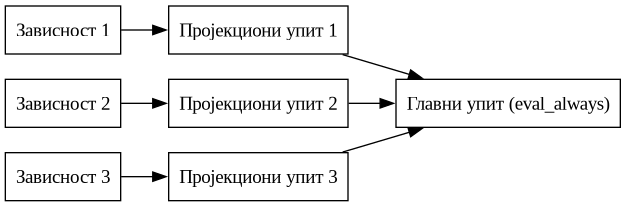
\includegraphics[width=4in, height=1.4in]{assets/images/projection_query.png}
\end{center}
\caption{Употреба "eval\_always" модификатора у пројекционом шаблону}
\label{lst:projection_query}
\end{listing}
\subsection{Типизирана међурепрезентација високог \\ нивоа (ТМВН) - Typed HIR (THIR)}

Типизирана међурепрезентација високог нивоа је међурепрезентација изворног кода која настаје допуном стабла типовима.
За разлику од \verb|HIR| међурепрезентације, ТМВН садржи само тела тј. извршни код. То значи да ТМВН 
не садржи репрезентацију ставки као што су структуре (\verb|struct|) и особине (\verb|traits|). Свако тело у овој репрезентацији
се чува приверемено у меморији и одбачено чим више није потребно. Ово је битна дистинкција у доносу на \verb|HIR| где се репрезентација 
чува током целокупног процеса компилације. Додатно, аутоматска референцирања и дереференцирања су експлицитна, позиви метода и 
преклопљени оператори су претворени у обичне позиве функција. Уништење опсега је у овој репрезентацији експлицитно.
Изрази, искази и клаузуле \verb|match| одредбе се чувају посебно.

\subsubsection{Безбедност}

Поједностављивањем изворног кода сажима се број различитих начина да се исти код напише и смањује раздаљину између 
кода који се анализира (АСТ) и кода који се извршава (битцоде).
Управо тај мањак инструкционе комплексности чини типизирану међурепрезентацију значајну у провери безбедности. 
Провере безбедности се налазе у модулу \verb|check_unsafety|.
Алгоритам пролази кроз тело функције и све њене анонимне функције пратећи да ли је небезбедном \verb|unsafe| контексту.
Уколико се небезбедан код позива ван небезбедног (\verb|unsafe|) блока грешка ће бити приказана. Алгоритам такође води рачуна да ли 
постоји небезбедан блок у коме се не користи небезбедан код. Ако постоји овакав блок компајлер ће приказати упозорење (\verb|lint|).

Додатак \ref{lst:safety_check} приказује исечак главне функције која је одговорна за опсег безбедности. 
На основу \verb|LocalDefId| добавља се тело у ТМВН међурепрезентацији. Потом се на основу истог 
идентификатора евалуира \verb|HirId| уз помоћ којег се врши упит над \verb|HIR|-ом чиме се открива почетни контекст безбедности.
Структура \verb|UnsafeVisitor| користи ТМВН тело, на основу ког спроводи претходно објашњен алгоритам. Може се приметити 
да се овде инцијализује вектор упозорења која се приказују уколико се небезбедан код не користи у небезбедном контексту.

\subsubsection{Провера шаблона}
\verb|Rust| језик поседује карактеристику да уколико се користи провера шаблона (\verb|pattern matching|), свака могућа 
варијација шаблона мора бити обрађена (има одговарајућу логику) тј. провера штаблона је исцрпна \ref{lst:pattern_matching}.
Проверу да ли је исцрпност задовољена извршава ТМВН. У провере шаблона спадају изрази \verb|match|, \verb|if let|, \verb|while let|,
\verb|let else|, \verb|let|, па чак и аргументи функција. Поред исцрпности, проверава се и корисност шаблона. Корисност одговара на питање 
да ли је неко гранање редудантно. Ово је вредно кориснику језика јер скреће пажњу да је неки сегмент изворног кода недостижан. 

\begin{listing}[H]
\begin{minted}{rust}
pub enum IpAddrKind { V4, V6, }
fn main() {
    let x = IpAddrKind::V4;
    match x {
        IpAddrKind::V4 => println!("Ovo je IPv4 adresa."), 
        IpAddrKind::V6 => println!("Ovo je IPv6 adresa.") 
        // Da je postojao IpAddrKind::V7 Rust bi zahtevao 
        // da i ta varijanta bude obradjena.
    }}
\end{minted}
\caption{Провера шаблона}
\label{lst:pattern_matching}
\end{listing}
\subsection{Medjureprezentacija srednjeg nivoa (MSN) - Mid-Level Intermediate Representation (MIR)}

Koncept medjureprezentacije srednjeg nivoa nije postojao od samog nastanka kompajlera. Prvobitno je koristio apstraktno sintaksno stablo 
iz inicijalnog parsiranja sve do finalne generacije bitkoda. Ovaj metod je dovodio do brojnih problema. Apstraktno sintaksno stablo i reprezentacija 
visokog nivoa su izgledom veoma slični izvornom kodu. Prevođenje sintaktičkog šećera na osnovni konstrukt nije imalo predodređeno mesto za čuvanje. 
Stoga svaka faza koja je morala da rasuđuje nešto na osnovu koda (npr. provera tipova, generisanje koda) je morala da simulira prevođenje od početka.
Sa obzirom da bi svaka faza morala biti upoznata sa svakim specijalnim slučajem prevođenja, krajnji rezultat uprošćavanja šećera bi činilo kompajler 
kompleksnijim, a ne jednostavnijim. Rasuđivanje kontrole toka preko apstraktnog sintaksnog stabla je veoma kompleksno. Graf kontrole toka se kreirao
iznad ASS-a, koristo se za analizu ali ne i tokom prevođenja, čime se analiziran graf kontrole toka nije morao podudarati sa grafom kontrole toka generisanog koda. 
Postojala su brojna mesta na kojima bi bilo efikasno upotrebiti Rust specifično znanje za izvršavanje optimizacija gde bi postojanje srednjeg sloja značajno pomoglo.
Migriranje od LLVM-a je bilo praktično nemoguće jer je semantika Rust jezika spojena sa korakom prevođenja u LLVM medjureprezentaciju.
Formalni dokazi su jedan od načina na koji bi Rust voleo da garantuje bezbednost, i samim time prethodno navedena, uvek promenljiva 
osnova nije podobna za ovaj posao.

Naime, uvođenje još jedne međureprezentacije ne dolazi bez mana. Konvertovanje iz ASS-a u MSN uvodi dodatno vreme prilikom kompajliranja. Više truda je potrebno 
da bi se kreirale kvalitetne poruke o problemima unutar koda jer je MSN značajno drugačije strukture od onoga što je korisnik uneo.

\subsubsection{Graf kontrole toka}

Danas, srednju medjureprezentaciju čini skup fajlova (kada se potraži od kompajlera) gde svaki opisuje izvršavanje jedne funkcije i direktno je vezan za graf kontrole toka. Graf kontrole toka je 
struktuiran kao grupa osnovnih blokova koji su povezani granama. Ključna ideja bloka jeste da je to grupa naredbi (iskaza) 
koja se izvršava zajedno. Svaki put kada se granom dodje do novog bloka, sve naredbe tog bloka moraju da se izvrše, pa tek onda postoji mogućnost 
da se grana dalje. Poslednja nareba unutar bloka se naziva terminator. Brojni izrazi \ref{lst:block_code} koji se koriste u Rust jeziku se kompajliraju na 
više osnovnih blokova \ref{lst:block_block}.

\begin{listing}[H]
\begin{minted}{rust}
a = 1;
if some_variable {
    b = 1;
} else {
    c = 1;
}
d = 1;
\end{minted}
\caption{Isečak koda koji se prevodi u više osnovnih blokova}
\label{lst:block_code}
\end{listing}


\begin{listing}[H]
\begin{minted}{text}
BB0: {
    a = 1;
    if some_variable {
        goto BB1;
    } else {
        goto BB2;
    }
}
BB1: {
    b = 1;
    goto BB3;
}
BB2: {
    c = 1;
    goto BB3;
}
BB3: {
    d = 1;
    ...
}
\end{minted}
\caption{Isečak koda u formi osnovih blokova}
\label{lst:block_block}
\end{listing}

Stek (\verb|Stack|) je LIFO (\verb|Last in First Out|) struktura podataka koju kompajler koristi da skladišti argumente funkcija,
lokalne promenljive i privremene promenljive. U MSN reprezentaciji memorijske lokacije na steku su identifikovane pomoću indeksa. 
Indeks se označava celobrojnom vrednošću koju prethodi donja crta (npr. \verb|_1|, \verb|_2|). Indeks \verb|_0| je specijalan, u njemu
se skladišti povratna vrednost. Mesta su izrazi koji identifikuju lokaciju u memoriji. Mesto može biti sam indeks (\verb|_1|) ili može biti
projekcija (\verb|_1.polje|). Projekcije su polja ili druge konstrukcije koje proizilaze iz mesta. Pristup polju je projekcija, za \verb|_1.polje|, \verb|_1| je mesto dok je \verb|polje| projekcioni element.
Dereferenciranje je takođe projekcija, za \verb|*_1|, \verb|_1| je mesto dok je \verb|*| projekcioni element. 
Desne vrednosti (\verb|RValues|) su izrazi koji generišu vrednost. Zovu se desne vrednosti zato što 
stoje sa desne strane operatora dodele (\verb|=|). Operandi su argumenti desne vrednosti. Argument može biti konstanta ili mesto (kao što je \verb|_1|).

Strukturu srednje medjureprezentacije je najlakše razumeti prevodjenjem jednostavnih programa poput \ref{lst:snippet-before-mir}. U dodatku \ref{lst:unoptimized-mir} se nalazi neoptimizovana njegova srednja medjureprezentacija. Glavna razlika izmedju optimizovane i neoptimizovanje srednje medjureprezentacije jeste to što neoptimizovana medjureprezentacija sadrži eksplicitne iskaze \verb|StorageLive| i \verb|StorageDead| unutar osnovnih blokova. Iskaz \verb|StorageLive| pruža informaciju da je promenljiva navedena u iskazu živa tj.
da ju je moguće koristiti u daljem izvršavanju. Iskaz \verb|StorageDead| pruža informaciju da je promenljiva navedena u iskazu mrtva
tj. nije je više moguće koristiti. Samim time ovo se pokazuje kao pravo mesto da se sprovodi dealokacija memorije.
Jedina informacija koju srednja reprezentacija ne zna eksplicitno jeste da li se dogodio prenos vlasništva. Ovu informaciju dobija na osnovu tipa promenljive.

\begin{listing}[H]
\begin{minted}{text}
fn main() {
    let mut vec = Vec::new();
    vec.push(1);
    vec.push(2);
}
\end{minted}
\caption{Isečak koda koji se prevodi u MSN}
\label{lst:snippet-before-mir}
\end{listing}

\subsubsection{Optimizacija koda u MSN-u}

Reprezentacija srednjeg nivoa u Rust kompajleru igra ključnu ulogu u optimizaciji koda pre njegove predaje LLVM bekendu. 
Generiše se iz TMVN-a i fokusira se isključivo na izvršni kod. Jedna od glavnih prednosti MSN-a je omogućavanje optimizacija specifičnih za Rust koje bi bilo teško 
sprovesti direktno na nivou LLVM IR-a. MSN pruža osnovu za analizu bezbedne primene optimizacija, 
jasno razdvajajući semantiku jezika od LLVM bekenda. MSN teži da pojednostavi reprezentaciju koda, potencijalno olakšavajući formalne dokaze u budućnosti.

Proces generisanja MSN-a rekurzivno obrađuje izraze iz TMVN-a. Odličan primer optimizacije i pojednostavljenja koje MSN omogućava je 
transformacija petlji. Na primer, \verb|for| petlja, koja se u ranijoj fazi MVN-a može svodi na \verb|while let| konstrukciju,
u MSN-u inicijalno biva transformisana u ekvivalentnu \verb|loop| petlju sa \verb|match| izrazom unutar nje:

\begin{minted}{rust}
let mut iterator = IntoIterator::into_iter(vec);
loop {
    match Iterator::next(&mut iterator){
        Some(elem) => process(elem),
        None => break,
    }
}
\end{minted}

Ova struktura preslikava semantiku \verb|while let|, ali MSN ide korak dalje u pojednostavljenju kontrole toka. Uvode se eksplicitne \verb|goto| 
naredbe i labele. Iako je \verb|goto| ključna reč koja nije dozvoljena u izvornom Rust kodu zbog potencijalnog narušavanja čitljivosti i 
otežanog praćenja toka izvršavanja u kompleksnim programima, u internoj reprezentaciji poput MSN-a on svodi petlje i grananja na najosnovnije 
operacije skoka. Ovo čini graf kontrole toka eksplicitnim i lakšim za analizu i dalju transformaciju od strane kompajlera. 
Petlja iz prethodnog primera sada izgleda ovako:

\begin{minted}{rust}
let mut iterator = IntoIterator::into_iter(vec);

loop: 
    match Iterator::next(&mut iterator) {
        Some(elem) => { process(elem); goto loop; } 
        None => { goto break; } 
    }

break: 
\end{minted}

Poslednji korak u ovom primeru je pojednostavljenje \verb|match| izraza, koji je i dalje relativno kompleksna sintaktička celina. 
Dok \verb|match| u izvornom kodu grupiše proveru obrasca i pristup podacima unutar njega, 
MSN ga razdvaja radi veće granularnosti i jednostavnosti osnovnih operacija. 
Uvodi se primitivna \verb|switch| naredba (koja nije dostupna u izvornom Rust-u) koja se bavi isključivo proverom diskriminante 
(da li je rezultat \verb|Some| ili \verb|None|). Pristup podacima unutar varijante 
(izdvajanje vrednosti \verb|elem| iz \verb|Some|) obavlja se kao zasebna operacija unutar odgovarajuće grane kontrole toka:

\break

\begin{minted}{rust}
let mut iterator = IntoIterator::into_iter(vec);

loop:
    let tmp = Iterator::next(&mut iterator); 
    
    switch tmp { 
        Some => { 
            let elem = (tmp as Some).0; 
            process(elem); 
            goto loop; 
        }
        None => { 
            goto break; 
        }
    }
    
break:
\end{minted}


Veoma je često da prilikom \verb|debug|-ovanja srednje reprezentacije potreban prikaz samo jedne funkcije
umesto celokupnog prevoda. Za prikaz celokupnog izlaza koristi se \verb|all| filter, dok ako je neka pojedinačna funkcija od interesovanja
njeno ime.

\begin{listing}[H]
\begin{minted}{bash}
cargo rustc -- -Z dump-mir=[filter] -Z dump-mir-graphviz
\end{minted}
\caption{Ispis i prikaz MSN-a}
\label{lst:mir_print}
\end{listing}

\subsubsection{Neleksički životni vekovi}

Pozajmljivač (\verb|borrow-checker|) nalaže da se pozajmljena vrednost ne može mutirati niti joj se može promeniti vlasništvo. Svaki put kada se vrednost pozajmi kreira se životni vek njene reference. 
Životni vek reference se odnosi na mesto koda gde bi se referenca mogla koristiti. Kompajler će se potruditi da evaluira najmanji opseg koji pokriva svako potencijalno korišćenje reference.
Životni vek može da se odnosi i na vrednost i na referencu. Da bi bilo jasno o čemu se govori, životni vek će se odnositi na životni vek reference, dok će se opseg odnositi na životni vek vrednosti \ref{lst:scope-lifetime}.

\begin{listing}[H]
\begin{minted}{rust}
fn foo() {
    let mut data = vec!['a', 'b', 'c'];    // --+ 'opseg
    capitalize(&mut data[..]);             //   |
//  ^~~~~~~~~~~~~~~~~~~~~~~~~ 'životni vek //   |
    data.push('d');                        //   |
    data.push('e');                        //   |
    data.push('f');                        //   |
} // <------------------------------------------+
\end{minted}
\caption{Opseg i životni vek}
\label{lst:scope-lifetime}
\end{listing}

\break

Leksički (statički) životni vek se određuje na osnovu strukture programa. U primeru \ref{lst:lexical-lifetime} definiše se mutabilna referenca nad vektorom \verb|data|.
Referencu je moguće koristiti u celokupnom opsegu funkcije, stoga opseg funkcije čini njen životni vek. To znači da su pozivi \verb|push| greška jer se dešavaju tokom životnog veka
reference.

\begin{listing}[H]
\begin{minted}{rust}
fn bar() {
    let mut data = vec!['a', 'b', 'c'];
    let slice = &mut data[..]; // <-+ 'životni vek
    capitalize(slice);         //   |
    data.push('d'); // GREŠKA!  //   |
    data.push('e'); // GREŠKA!  //   |
    data.push('f'); // GREŠKA!  //   |
} // <------------------------------+
\end{minted}
\caption{Problem kod leksičkog životnog veka}
\label{lst:lexical-lifetime}
\end{listing}

Ovakvi problemi su se mogli zaobići enkapsuliranjem reference u blok \ref{lst:lexical-lifetime-ok}. Ovaj zaobilazni put je možda logičan ali izgleda veštački i otežava korišćenje jezika. 

\begin{listing}[H]
\begin{minted}{rust}
fn bar() {
    let mut data = vec!['a', 'b', 'c'];
    {
        let slice = &mut data[..]; // <-+ 'životni vek
        capitalize(slice);         //   |
    } // <------------------------------+
    data.push('d'); // OK
    data.push('e'); // OK
    data.push('f'); // OK
}
\end{minted}
\caption{Opseg i životni vek}
\label{lst:lexical-lifetime-ok}
\end{listing}

Prethodni primer je jedan od najjednostavnijih problema leksičkog životnog veka, napredniji problemi postaju teži za uočavanje i još teži za razumevanje.
Uvođenjem MSN-a dobijen je efikasan način evaluacije životnog veka na osnovu kontrole toka grafa gde se granularno određuje životni vek reference \ref{lst:dynamic-lifetime} (ovako \verb|Rust| radi danas).

\begin{listing}[H]
\begin{minted}{rust}
fn bar() {
    let mut data = vec!['a', 'b', 'c'];
    let slice = &mut data[..];   // <-+ 'životni vek
    capitalize(slice);           //   |
    // <------------------------------+
    data.push('d'); // OK
    data.push('e'); // OK
    data.push('f'); // OK
} 
\end{minted}
\caption{Dinamički životni vek}
\label{lst:dynamic-lifetime}
\end{listing}
\section{Zaključak}

Ovaj master rad pružio je uvid u arhitekturu Rust kompajlera, sa posebnim fokusom na ključnu ulogu koju igraju međureprezentacije izvornog koda u procesu prevođenja. 
Počevši od osnova Rust jezika, njegovog ekosistema sa alatom Cargo, i oslanjanja na LLVM projekat za generisanje optimizovanog mašinskog koda, 
analiziran je sam proces kompajliranja.

Centralni deo rada detaljno je istražio putanju koda kroz seriju međureprezentacija. 
Pokazano je kako se od inicijalnog toka tokena i ASS-a, preko MVN-a koji vrši pojednostavljenje sintakse i predstavlja platformu za prelazak sa \verb|pipeline|
kompajlerske arhitekture na arhitekturu zasnovanu na upitima, dolazi do TMVN-a gde se integrišu informacije o tipovima ključne za bezbednost 
i analizu šablona.

Posebna pažnja posvećena je međureprezentaciji srednjeg nivoa (MSN). Naglašena je njena uloga kao eksplicitnog grafa kontrole toka,
što je čini fundamentalnom za implementaciju Rust-ovih garancija memorijske bezbednosti kroz proveru pozajmljivanja i neleksičke životne vekove.
Takođe, MSN služi kao osnova za važne Rust-specifične optimizacije, pre nego što se dalja optimizacija i generisanje koda prepuste LLVM-u.

Kroz ovu analizu, demonstrirano je da višefazni pristup sa pažljivo dizajniranim međureprezentacijama nije samo tehnički detalj,
već suštinski mehanizam koji omogućava Rustu da istovremeno postigne svoje glavne ciljeve: memorijsku bezbednost bez sakupljača smeća,
visoke performanse koje pariraju C/C++-u, i izražajnost jezika sa modernim karakteristikama. Složenost kompajlera je efikasno modularizovana,
omogućavajući rigorozne provere i optimizacije na najpogodnijem nivou apstrakcije. Razumevanje ovih internih faza ključno je za dalje unapređenje kompajlera,
razvoj alata za analizu koda i dublje shvatanje samog jezika Rust.
\section{Literatura}

\begin{thebibliography}
    \raggedright
\bibitem{msrc} 
    MSRC, “A proactive approach to more secure code | MSRC Blog | 
    Microsoft Security Response Center,” Microsoft.com, Jul. 16, 2019. 
    \url{https://msrc.microsoft.com/blog/2019/07/a-proactive-approach-to-more-secure-code/} 
    (pristupljeno Sep. 08, 2024).

    \bibitem{parsing} 
    “Parsing” Rochester.edu, 2024.
    \url{https://www.cs.rochester.edu/u/nelson/courses/csc_173/grammars/parsing.html#:~:text=Recursive%2Ddescent%20parsing%20is%20one,non%2Dterminal%20with%20a%20procedure} 
    (pristupljeno Sep. 21, 2024).

    \bibitem{dragonbook} 
    A. V. Aho, M. S. Lam, R. Sethi, and J. D. Ullman, \emph{Compilers: Principles, Techniques, and Tools}, 2nd ed. Boston, MA, USA: Addison-Wesley, 2006.

    \bibitem{rust-guide} 
    “Getting Started - Rust Compiler Development Guide,” Rust-lang.org, 2024. 
    \url{https://rustc-dev-guide.rust-lang.org/getting-started.html} (pristupljeno Sep. 28, 2024).

    \bibitem{rust-reference}
    “Introduction - The Rust Reference,” Rust-lang.org, 2015. 
    \url{https://doc.rust-lang.org/reference/introduction.html} (pristupljeno Sep. 29, 2024).
    
    \bibitem{rustonomicon}
    “Meet Safe and Unsafe - The Rustonomicon,” Rust-lang.org, 2024. 
    \url{https://doc.rust-lang.org/nomicon/meet-safe-and-unsafe.html} (pristupljeno Sep. 29, 2024).

    \bibitem{editions}
    “What are editions? - The Rust Edition Guide,” Rust-lang.org, 2024.
    \url{https://doc.rust-lang.org/edition-guide/editions/} (pristupljeno Okt. 03, 2024).

    \bibitem{unstable}
    “The Unstable Book - The Rust Unstable Book,” Rust-lang.org, 2024. 
    \url{https://doc.rust-lang.org/unstable-book/index.html} (pristupljeno Okt. 06, 2024).

    \bibitem{unstable-flags}
    Li, Chenghao, et al. “Demystifying Compiler Unstable Feature Usage and Impacts in the Rust Ecosystem.” 26 Oct. 2023. arXiv, Pristupljeno 6 Oct. 2024. 

    \bibitem{rust-language}
    Bugden W, Alahmar A. Rust: The programming language for safety and performance. arXiv preprint arXiv:2206.05503. 2022 Jun 11.

    \bibitem{supply-chain}
    P. Mainardi, “The Rising Threat of Software Supply Chain Attacks: Managing Dependencies of Open Source projects,” Linuxfoundation.eu, Aug. 15, 2023.
    \url{https://linuxfoundation.eu/newsroom/the-rising-threat-of-software-supply-chain-attacks-managing-dependencies-of-open-source-projects} (pristupljeno Okt. 20, 2024).

    \bibitem{oss-architecture}
    “The Architecture of Open Source Applications (Volume 1)LLVM,” Aosabook.org, 2024. 
    \url{https://aosabook.org/en/v1/llvm.html} (pristupljeno Nov. 04, 2024).

    \bibitem{llvm}
    “The LLVM Compiler Infrastructure Project,” Llvm.org, 2024. 
    \url{https://llvm.org/} (pristupljeno Nov. 04, 2024).
\end{thebibliography}
\section{Додатак 1}

\begin{listing}[H]
\begin{minted}{rust}
#[proc_macro_attribute]
pub fn expand_body(_attr: TokenStream, _item: TokenStream) -> TokenStream {
    let fun = format!("fn missing_body() 
    {{ println!(\"I'm not missing body anymore.\"); }}");

    let stream: TokenStream = fun.parse().unwrap();

    stream
}

#[expand_body]
fn missing_body();

fn main() {
    missing_body();
}
\end{minted}
\caption{Додавање тела функције уз помоћ макроа}
\label{lst:bonus_body_expand}
\end{listing}

\clearpage

\section{Додатак 2}
\begin{listing}[H]
\begin{minted}{rust}
fn try_mark_green(tcx, current_node) -> bool {
// Fetch the inputs to `current_node`, i.e. get the nodes that the direct
// edges from `node` lead to.
let dependencies = tcx.dep_graph.get_dependencies_of(current_node);
// Now check all the inputs for changes
for dependency in dependencies {
match tcx.dep_graph.get_node_color(dependency) {
Green => {
// This input has already been checked before and it has not
// changed; so we can go on to check the next one
}
Red => {
// We found an input that has changed. We cannot mark
// `current_node` as green without re-running the corresponding query.
    return false
}
Unknown => {
// This is the first time we look at this node. Let's try
// to mark it green by calling try_mark_green() recursively.
    if try_mark_green(tcx, dependency) {
// We successfully marked the input as green, on to the next.
    } else {
// We could *not* mark the input as green. This means we
// don't know if its value has changed. In order to find
// out, we re-run the corresponding query now!
        tcx.run_query_for(dependency);
// Fetch and check the node color again. Running the query
// has forced it to either red (if it yielded a different
// result than we have in the cache) or green (if it
// yielded the same result).
        match tcx.dep_graph.get_node_color(dependency) {
            Red => {
// The input turned out to be red, so we cannot mark `current_node` as green.
                return false
            }
            Green => {
// Re-running the query paid off! The result is the same as before, 
// so this particular input does not invalidate `current_node`.
            }
            Unknown => {
// There is no way a node has no color after re-running the query.
                panic!("unreachable") } } } } } }
tcx.dep_graph.mark_green(current_node);
true }
\end{minted}
\caption{Имплементација алгоритма "try-mark-green"}
\label{lst:bonus_try_mark_green}
\end{listing}

\section{Додатак 3}

\begin{listing}[H]
\begin{minted}{rust}
let Ok((thir, expr)) = tcx.thir_body(def) else { return };
// Runs all other queries that depend on THIR.
tcx.ensure_with_value().mir_built(def);
let thir = &thir.steal();
// If `thir` is empty, a type error occurred, skip this body.
if thir.exprs.is_empty() {
    return;
}

let hir_id = tcx.local_def_id_to_hir_id(def);
let safety_context = tcx.hir().fn_sig_by_hir_id(hir_id)
.map_or(SafetyContext::Safe, |fn_sig| {
    if fn_sig.header.safety == hir::Safety::Unsafe {
        SafetyContext::UnsafeFn
    } else {
        SafetyContext::Safe
    }
});
let body_target_features = &tcx.body_codegen_attrs(def.to_def_id()).target_features;
let mut warnings = Vec::new();
let mut visitor = UnsafetyVisitor {
    tcx, thir, .  .  ., warnings: &mut warnings,
    suggest_unsafe_block: true,
};
visitor.visit_expr(&thir[expr]);

warnings.sort_by_key(|w| w.block_span);
for UnusedUnsafeWarning { hir_id, block_span, enclosing_unsafe } in warnings {
    let block_span = tcx.sess.source_map().guess_head_span(block_span);
    tcx.emit_node_span_lint(
        UNUSED_UNSAFE,
        hir_id,
        block_span,
        UnusedUnsafe { span: block_span, enclosing: enclosing_unsafe },
    );}
\end{minted}
\caption{Провера безбедности}
\label{lst:safety_check}
\end{listing}


\section{Додатак 4}


\begin{listing}[H]
\begin{minted}{text}
fn main() -> () {
    let mut _0: ();
    let mut _1: std::vec::Vec<i32>;
    let _2: ();
    let mut _3: &mut std::vec::Vec<i32>;
    let _4: ();
    let mut _5: &mut std::vec::Vec<i32>;
    scope 1 {
        debug vec => _1;
    }
    bb0: {
        StorageLive(_1);
        _1 = Vec::<i32>::new() -> [return: bb1, unwind continue];
    }
    bb1: {
        StorageLive(_2);
        StorageLive(_3);
        _3 = &mut _1;
        _2 = Vec::<i32>::push(move _3, const 1_i32) -> [return: bb2, unwind: bb5];
    }
    bb2: {
        StorageDead(_3);
        StorageDead(_2);
        StorageLive(_4);
        StorageLive(_5);
        _5 = &mut _1;
        _4 = Vec::<i32>::push(move _5, const 2_i32) -> [return: bb3, unwind: bb5];
    }
    bb3: {
        StorageDead(_5);
        StorageDead(_4);
        _0 = const ();
        drop(_1) -> [return: bb4, unwind: bb6];
    }
    bb4: {
        StorageDead(_1);
        return;
    }
    bb5 (cleanup): {
        drop(_1) -> [return: bb6, unwind terminate(cleanup)];
    }
    bb6 (cleanup): {
        resume;
    }
}
\end{minted}
\caption{Неоптимизована МСН}
\label{lst:unoptimized-mir}
\end{listing}

\section{Подаци о кандидату}


Кандидат Алекса Бајат рођен је 2001. године у Новом Саду. Завршио је природно-математички смер на енглеском језику 
у гимназији "Јован Јовановић Змај" 2019. године. Током све четири године гимназије успешно је похађао 
"Центар за младе таленте" компаније \verb|Schneider Electric|.  Године 2019. уписао је Факултет 
Техничких Наука у Новом Саду, где је испунио све обавезе и положио све испите предвиђене 
студијским програмом са просечном оценом 9.03. 

\end{document}
